\history{Date of publication xxxx 00, 0000, date of current version xxxx 00, 0000.}
\doi{10.1109/ACCESS.2020.DOI}

\title{Fast and robust low-rank approximation for high-dimensional seismic data reconstruction}
%\author{\uppercase{Juan Wu}\authorrefmark{1},
%\uppercase{Second B. Author\authorrefmark{2}, and Y. Chen}.\authorrefmark{3},
%\IEEEmembership{Member, IEEE}}
%\address[1]{National Institute of Standards and 
%Technology, Boulder, CO 80305 USA (e-mail: author@boulder.nist.gov)}
%\address[2]{Department of Physics, Colorado State University, Fort Collins, 
%CO 80523 USA (e-mail: author@lamar.colostate.edu)}
%\address[3]{Electrical Engineering Department, University of Colorado, Boulder, CO 
%80309 USA}


%\markboth
%{Author \headeretal: Preparation of Papers for IEEE TRANSACTIONS and JOURNALS}
%{Author \headeretal: Preparation of Papers for IEEE TRANSACTIONS and JOURNALS}

\author{Juan Wu\footnotemark[1], Min Bai\footnotemark[1], Dong Zhang\footnotemark[2], Hang Wang\footnotemark[3], Guangtan Huang \footnotemark[3], and Yangkang Chen\footnotemark[3] }

%\author{*}
\address{
\footnotemark[1]Key Laboratory of Exploration Technology for Oil and Gas Resources of Ministry of Education\\
Yangtze University\\
Wuhan 430100, China\\
%yangkang.chen@zju.edu.cn \\
\footnotemark[2] Faculty of Applied Sciences \\
Delft University of Technology \\
Lorentzweg 1, Delft, Netherlands, 2628CJ  \\
%d.zhang-3@tudelft.nl \\ 
\footnotemark[3] School of Earth Sciences \\
Zhejiang University \\
Hangzhou, Zhejiang, 310027 \\
}

\corresp{Corresponding author: M. Bai (e-mail: baimin2016@126.com).}
\tfootnote{This research is sponsored by the National Natural Science Foundation of China (Nos. \new{41904110,}41704121), \new{the China Postdoctoral Science Foundation (No. 2019M662567), and the Postdoctoral Science Foundation of Hubei Province.}}


\def\thevol{8}
\def\myyear{2020}

\begin{abstract}
Five-dimensional (5D) seismic data reconstruction becomes more appealing in recent years because it takes advantage of five physical dimensions of the seismic data \old{for reconstruction }and can reconstruct data with large gap. The low-rank approximation approach is one of the most effective methods for reconstructing 5D dataset. However, the main disadvantage of the low-rank approximation method is its low computational efficiency because of many singular value decompositions (SVD) of the block Hankel\new{/Toeplitz} matrix in the frequency domain. In this paper, we develop an SVD-free low-rank approximation method for efficient and effective reconstruction and denoising of the seismic data that \old{contains}\new{contain} four spatial dimensions. Our SVD-free rank constraint model is based on an alternating minimization strategy, which updates one variable each time while fixes the other two. For each update, we only need to solve a linear least-squares problem with much less expensive QR factorization. The SVD-based and SVD-free low-rank approximation \new{methods} in the singular spectrum analysis (SSA) framework are compared in detail, regarding the reconstruction performance and computational cost. The comparison shows that the SVD-free low-rank approximation method can obtain similar reconstruction performance as the SVD-based method but with a large computational speed up.
\end{abstract}

\begin{keywords}
Multidimensional seismic data, \old{lowrank}\new{low-rank} approximation, seismic data processing, \new{seismic reconstruction, matrix completion}
\end{keywords}

\titlepgskip=-15pt

\maketitle

\section{Introduction}
\label{sec:introduction}

Data reconstruction is extremely important during the entire seismic processing chain due to the fact that our acquired data are never complete and regular in spatial dimensions. More specifically, abundant physical and economic restrictions happen throughout the acquisition phase resulting in data incompletion, e.g., feathering, near-offset gap, cross-line under-sampling in towed marine streamer acquisition and obstacles, terrain restrictions in land acquisition \cite{ronen,spitz1991,canning1996,fomel2002pwd,fomel2003,abmapocs,herrmann2008non,mostafa2010,mostafa2013,wang2011recovery,shuwei2016cs,shaohuan2016gap,yangkang2016irr5d,amir2017ieee}. Incompletely and irregularly recorded seismic data always have severely negative effects on the subsequent data processing work flow, such as surface related multiple elimination, velocity analysis, full waveform inversion, wave equation migration, time-frequency analysis, amplitude versus offset inversion and seismic interpretation \cite{verschuure1991,shuwei20153,shuwei2016vscan,liuwei2016dealiase}.


Seismic data reconstruction, therefore, has drawn a large amount of attention from both academia and industry in the past several decades. It can be divided into two very basic categories: model-driven methods and data-driven methods. Although model driven methods are powerful and could be highly accurate, \old{a prior}\new{a-priori} knowledge about the model needs to be provided, while it is not simple at all to build an accurate model. In addition to \old{a prior}\new{a-priori} knowledge about the model, computational cost is another big issue for model-driven reconstruction methods. On the contrary, data-driven reconstruction methods are significantly popular among seismic exploration community because of their higher efficiency and less dependency on model. Usually, simple mathematical assumptions are utilized in data-driven methods for interpolating seismic data, which turns out to be more solid and effective. Since the last decade, a majority of researchers have made lots of efforts to investigate all different types of data-driven reconstruction methods. In recent years, dictionary learning and machine learning are applied to the reconstruction of 5D simple data \cite{YuSiwei2015, YuSiwei2016, Jia2017, amir2017sp,amir2017geo, Jia2018}. Data driven tight frame (DDTF) is a kind of dictionary-learning method, which can simultaneously denoise and interpolate 5D seismic data \cite{YuSiwei2015}. In DDTF, a sparsity-promoting algorithm is used to build the dictionary which can represent the observed data and estimate the complete data. \cite{Jia2017} combined the DDTF with a classic machine learning method named support vector regression (SVR) to optimize the learning, which obtained better performance than the Gauss SVR method. With the continuous improvement of intelligent methods, learning-based 5D data reconstruction will be a hot research topic in the future.

In the seismic data processing literature, it is also noticed that the challenge of random noise always comes along with data reconstruction. In general, random noise suppression is of significant importance for both increasing the signal-to-noise ratio ($SNR$) \cite{yangkang2015ortho} and improving seismic data reconstruction performance. Random noise are capable of severely affecting the final performances of reconstruction methods, and thus, much attention has been drawn to random noise attenuation algorithms \cite{guochang2012,fxnaghizadeh,beckouche,yangkang2015ortho}. While most random noise attenuation approaches utilize the signal predictability, the irregularity of seismic data can directly influence this predictability and result in unsatisfactory denoising performance. Because of these mutual influences mentioned above between random noise suppression and data reconstruction, simultaneous reconstruction and denoising approaches are widely studied in \cite{oropezamssa}, \cite{gaomssa}, \cite{Gaogp}, \cite{gholami}, \cite{benfengpocs} and \cite{pmf}. Among all these approaches, low-rank approximation methods are most commonly studied. 

Meanwhile in recent years, simultaneous 5D seismic data reconstruction and denoising have become very popular due to the fact that it is capable of taking all physical dimensions of seismic data into consideration \cite{Liubin2004, Trad2007, Trad2009}, and thus, can take advantage of more data constraints and correlations to improve the reconstruction performance even at an extremely high data missing ratio. Especially when compared with 2D and 3D data cases, 5D data interpolation and denoising can always provide much better results. There exist two different categories for 5D interpolation: Fourier based approaches and low-rank approximation based approaches. Nowadays, 5D Fourier based interpolation methods have already become a standard for industry due to its stability and efficiency. Nevertheless, it is reported that the reconstruction performance of 5D Fourier based methods is less accurate than the low-rank approximation based approaches especially when dealing with curved events. On the other hand, low-rank approximation methods for simultaneous 5D seismic data reconstruction and denoising are widely studied during the last decade.

low-rank approximation approaches still have two subcategories: tensor based methods and block Hankel\new{/Toeplitz} matrix based methods. The first category regards multi-dimensional data as multi-linear arrays and applies dimensionality reduction on multi-linear arrays, in which some folding and unfolding operations are utilized. These methods are usually referred to as tensor completion. The other category transforms seismic data into multi-level block Hankel\new{/Toeplitz} matrix and a rank reduction algorithm can be used to recover the data, which can also be named multichannel singular spectrum analysis (MSSA) or Cadzow filtering. Although simultaneous 5D seismic data reconstruction and denoising via low-rank approximation becomes more attractive recently, there are still many challenges within this framework. \new{Major issues in low-rank approximation approaches for 5D data interpolation are \cite{Xie2017}: (1) high computational cost during SVD process, (2) the inevitable residual noise \cite{yangkang2016irr5d} and (3) the rank inconsistency problem \cite{yangkang2020odrr}}.  

Firstly, high computational cost during SVD process is the biggest problem we encounter to overcome especially for 5D dataset \cite{lu2015fast,jinkun2016}. Since our target multi-level block Hankel\new{/Toeplitz} matrix or tensor array tends to be extremely large, the truncated SVD process consumes huge amounts of time. Many researchers have made lots of efforts to solve this problem. \cite{oropezamssa} proposed to replace truncated SVD with randomized SVD to accelerate the MSSA based rank reduction method. \cite{gaomssa} introduced a fast rank reduction approach along four spacial dimensions based on Lanczos bidiagonalization. Instead of accelerated low-rank approximation for multi-level Hankel\new{/Toeplitz} matrix, \cite{pmf} presented a tensor completion based fast algorithm via parallel matrix factorization to speed up the 5D interpolation process. \new{Recently, \cite{jianjun2017five} developed a parallel square matrix factorization method for efficient 5D data reconstruction without SVD calculation, which however could be difficult in the implementation.}

Secondly, the recently discovered inevitable residual noise is another big issue preventing low-rank approximation approaches from having even better performance \cite{gavish2014optimal,trickett2015preserving,aharchaou2017singular,yatong2018gji}. Usually, conventional low-rank approximation methods can obtain reasonably good results while there are still amount of visible residual noise left, which is more severe for land seismic data. The reason behind is simply due to the incomplete decomposition between signals and noise. \cite{weilin2016} first noticed the inevitable residual noise during the truncated SVD process in MSSA for random noise attenuation and it is proved that the residual noise come from the signal-plus-noise subspace, which is decomposed by the truncated SVD. Therefore, damped MSSA is proposed to mitigate this noise leakage problem by introducing a damping factor to better decompose the signal and noise \cite{weilin2016}. Note that the later proposed double least-squares projection has more or less the similar concept with damped MSSA \cite{weilingieeedls}. \cite{dong} proposed a multi-step damped MSSA algorithm to further improve the SNR during reconstruction. \new{Straightforwardly, \cite{yangkang2016irr5d} extended damped MSSA to simultaneous 5D seismic data reconstruction and denoising in the condition with extremely noisy land seismic data. A much cleaner and more robust 5D interpolation result can be obtained by imposing more accurate signal and noise space decomposition.} In addition, \cite{dong2017} presented a novel hybrid rank sparsity constraint on seismic data to improve the interpolation performance with less residual noise. This hybrid constraint can take advantage of both constraints to upgrade the final results. \wen{A similar strategy hybrid model was proposed in \cite{yufeng2017} based on a different framework called the three-operator proximal splitting scheme.} 

Thirdly, an easily neglected but highly important issue is the rank inconsistency problem during low-rank approximation \cite{yangkangelra,shaohuan2017gji,baimin2018cg}. Seismic events are usually complicated, therefore, it is difficult to select a single appropriate rank value for the whole dataset. If the rank is chosen too large, little noise will be removed and if the rank is too small, even useful signals are lost. An effective strategy to mitigate this issue is to process the data within local windows, which better satisfies the basic linear assumption of low-rank approximation methods. However, it still fails due to highly nonstationary property of seismic data in both time and space, for example, when dealing with crossing events where the rank should be higher than other local windows. \cite{yangkangelra} proposed empirical low-rank approximation, in which the multi-dip data are decomposed to multiple single-dip data so that the optimal rank one can be applied to each local window. \new{More recently, \cite{yangkang2020odrr} developed an adaptive rank thresholding method to make the damped rank-reduction method suitable for local processing.}

In this paper, we address the first issue, i.e., the problem of low computational efficiency, of the low-rank approximation methods. We discuss an SVD-free low-rank approximation method for efficient and effective reconstruction and denoising of 5D seismic data that contains four spatial dimensions. Our SVD-free rank constraint model is based on an alternating minimization strategy, which updates one variable each time while fixing the other two. For each update, we only need to solve a linear least-squares problem with much more efficient QR factorization. We compare the performance of the traditional SVD-based and the proposed SVD-free low-rank approximation methods in detail. Extensive results show that the proposed SVD-free low-rank approximation method can obtain similar performance as the traditional SVD-based method, but with a much higher computing speed. The computational efficiency becomes more noticeable when the data size becomes larger. 


\section{low-rank approximation framework for 5D seismic data}
\wen{\subsection{The inverse problem}
The 5D reconstruction problem aims to solve the following inverse problem \cite{oropezamssa,stanton2013processing,gaomssa}:
\begin{equation}
\label{eq:5d}
\mathbf{D}^{obs}=\mathcal{S}\circ \mathbf{D}^{ideal},
\end{equation}
where $\mathbf{D}^{obs}$ denotes the observed data, $\mathbf{D}^{ideal}$ denotes the complete data, and $\mathcal{S}$ denotes the sampling operator,  which can be more specifically displayed as follows:
\begin{equation}
\mathcal{S}(i,j)=\left\{
\begin{array}{lr}
1, & for \ (i,j) \in \Omega\\             
0, & for \ (i,j) \notin \Omega
\end{array}
\right..
\end{equation}
$\Omega$ represents the subset of observed indices. $\mathcal{S}$ equals 1 at the observation point while 0 at the missing traces. $\circ$ denotes element-wise product. Both $\mathbf{D}^{obs}$ and $\mathbf{D}^{ideal}$ are considered in the frequency domain.} 

The inverse problem can be solved via the rank-reduction method, based on a weighted iterative algorithm \cite{oropezamssa,gaomssa}:
\begin{equation}
\label{eq:mssapocs}
\begin{split}
&\mathbf{D}_n=a_n \mathbf{D}_{obs} + (1-a_n) \mathcal{S}\circ \mathcal{M} \mathbf{D}_{n-1} + (1-\mathcal{S}) \circ\mathcal{M}\mathbf{D}_{n-1},\\
&\qquad n=1,2,3,\cdots,n_{max},
\end{split}
\end{equation}
where $\mathbf{D}_0=\mathbf{D}_{obs}$. The operator $\mathcal{M}$ represents the low-rank approximation operator that is based on \new{truncated singular value decomposition (TSVD)}\old{TSVD} for rank reduction.  $a_n$ is an iteration-dependent scalar that linearly decreases from $a_1=1$ to $a_{n_{max}}=0$.  The algorithm stops when either a maximum number of iterations $n_{max}$ has been reached or $\Arrowvert \mathbf{D}_n - \mathbf{D}_{n-1}\Arrowvert_F^2 \leq tol$. $tol$ denotes a very small tolerance value. In fact, equation \ref{eq:mssapocs} represents the general low-rank approximation for simultaneous seismic data reconstruction and denoising. Next, we will introduce the rank constraint model that is connected with the rank-reduction operator.

\subsection{The rank constraint model}
Presuming the original data matrix $\mathbf{X}$ is of low-rank structure, due to the theory of matrix completion, the randomly missing data can be reconstructed by a rank-minimizing model:
\begin{equation}
\label{eq:rank1}
\begin{split}
\min_{\mathbf{X}} & \quad \text{rank}(\mathbf{H} \mathbf{X}) \qquad s.t. \ \mathbf{X}_{i,j,k,l}=\mathbf{Y}_{i,j,k,l}\\
 & \text{for} \  (i,j,k,l) \in \Omega,
 \end{split}
\end{equation}
where $rank(\mathbf{H} \mathbf{X})$ is the number of non-zero singular values of $\mathbf{H} \mathbf{X}$. $\mathbf{H}$ denotes some mapping operations, for instance, the block Hankelization\new{/Toeplitization} operator in equation \ref{eq:hankelopt}. $\mathbf{Y}$ is the observed seismic data. \dlo{$\Omega$ represents the subset of observed indices.}

The constrained minimization problem in equation \ref{eq:rank1} can be converted to the unconstrained minimization problem in equation \ref{eq:rank2} by introducing the balancing parameter:
\begin{equation}
\label{eq:rank2}
\min_{\mathbf{X}} rank(\mathbf{H} \mathbf{X}) + \frac{1}{2} \mu \Arrowvert \mathbf{S}_{\Omega}(\mathbf{X}) -\mathbf{Y}\Arrowvert_F^2,
\end{equation}
where $\Arrowvert\cdot\Arrowvert_F$ denotes the Frobenius norm. $\mathbf{S}_{\Omega}$ denotes trace sampling. $\mu$ denotes balancing coefficient, which can balance the weight between rank constraint and data misfit. In practice, this balancing parameter is explicitly connected to the estimated rank value in the rank constraint. 

\dlo{Inspired by ? and ?, the conventional rank constraint model for 5D seismic data can be solved as follows: Take a block of 5D seismic data $\mathbf{D}_{time}(t,hx,hy,x,y)$ of $N_t$ by $N_{hx}$ by $N_{hy}$ by $N_x$ by $N_y$ samples $(t=1\cdots N_t, hx=1\cdots N_{hx}, hy=1\cdots N_{hy}, x=1\cdots N_x,y=1\cdots N_y)$ into consideration. The low-rank approximation works on seismic data as follows: first, the low-rank approximation directly transforms $\mathbf{D}_{time}(t,hx,hy,x,y)$ into $\mathbf{D}_{freq}(\omega,hx,hy,x,y), (\omega=1\cdots N_\omega)$ of complex values in the frequency domain. Each frequency slice in the data, at a specific frequency $\omega_0$, can be described by $\mathbf{D}(\omega_0)$. For simplicity, we drop the argument $\omega_0$ to avoid notational clutter. So now the 5D seismic data can be regarded as a number of 4D frequency data slices or matrices. }
The transformation of the 4D data matrix into a level-four block Hankel\new{/Toeplitz} matrix can be represented in operator notation as follows:
\begin{equation}
\label{eq:hankelopt}
\mathbf{M}=\mathcal{H}\mathbf{D},
\end{equation}
where $\mathcal{H}$ denotes the level-four block Hankelization\new{/Toeplitization} operator. \dlo{The detailed construction process of level-four Hankelization operator is elaborated in the Appendix A.}

Both missing traces and additive noise increase the rank of the matrix $\mathbf{M}$, which originally possesses low-rank structure. We assume that $\mathbf{M}$ has full rank, $rank(\mathbf{M})=J$ and the desired low-rank matrix $\mathbf{M}_K$ has deficient rank, $rank(\mathbf{M}_K)=K<J$. Therefore, the desired low-rank approximation can be obtained by a rank reduction method using truncated singular value decomposition (TSVD):
\begin{equation}
\label{eq:reductionopt}
\mathbf{M}_K=\mathbf{U}_K\mathbf{U}_K^H\mathbf{M}=\mathcal{R}_K\mathbf{M},
\end{equation} 
where we use $\mathcal{R}_K$ as the rank reduction operator via TSVD. $\mathbf{U}_K$ resulting from TSVD denotes the first $K$ singular vectors of matrix $\mathbf{M}$. The symbol $[\cdot]^H$ represents the conjugate transpose of a matrix. \new{Due to the TSVD step, the low-rank approximation method discussed in this paper can also be understood as a PCA method \cite{weilingieeedls}.}

After rank reduction, the filtered data can be recovered with random noise attenuated and missing traces reconstructed via properly averaging along the anti-diagonals of the target low-rank approximation matrix $\mathbf{M}_K$: 
\begin{equation}
\label{eq:mssaopt}
\hat{\mathbf{D}}=\mathcal{A}\mathbf{M}_{K}=\mathcal{A}\mathcal{R}_K\mathbf{M}=
\mathcal{A}\mathcal{R}_K\mathcal{H}\mathbf{D}=\mathcal{M}\mathbf{D},
\end{equation}
where $\mathcal{A}$ denotes the averaging operator. \dlo{The operator $\mathcal{M}$ represents the low-rank approximation operator that is based on TSVD for rank reduction.}

Here is a complete and detailed description of low-rank approximation framework for 5D seismic data. We adopt the following algorithm for reconstructing 5D noisy seismic data with missing traces:
\begin{algorithm}{LR}{\mathcal{S},\mathcal{F}_d,\mathbf{D}_{obs}(t,hx,hy,x,y),a_n,tol,N,F}
	\mathbf{D}_{obs}(w,hx,hy,x,y) \= \mathbf{D}_{obs}(t,hx,hy,x,y)\\
	 \text{by 1D forward FFT} \\
	\mathbf{D}_0 \= \mathbf{D}_{obs} \\
	\begin{FOR}{f \= 1, 2, \ldots, F} \\	
		\begin{FOR}{n \= 1, 2, \ldots, N} \\
			\mathbf{D}_n^f \= a_n \mathbf{D}_{obs}^f + (1-a_n) \mathcal{S} \circ \mathcal{F}_d \mathbf{D}_{n-1}^f\\
			 + (1-\mathcal{S}) \circ \mathcal{F}_d \mathbf{D}_{n-1}^f\\
			\begin{IF}{\Arrowvert \mathbf{D}_n^f - \mathbf{D}_{n-1}^f \Arrowvert_F^2 \leq tol} 
				\RETURN \mathbf{D}_n^f
			\end{IF}     
		\end{FOR} \\
		\RETURN \mathbf{D}_N^f
	\end{FOR}\\ 
	\RETURN \mathbf{D}_{recoverd}\\
	\mathbf{D}_{recoverd}(t,hx,hy,x,y) \= \mathbf{D}_{recoverd}(w,hx,hy,x,y) \\
	\text{by 1D inverse FFT}
\end{algorithm}
The iteration terminates after all $F$ frequencies are finished. For each frequency slice, the iteration terminates after $N$ iterations or upon reaching convergence to the specified tolerance $tol$.


\section{Fast and robust low-rank approximation approach}
Both conventional rank constraint and its solution are valid and robust, however, the computational cost is a major issue due to SVD in the low-rank approximation framework. SVD consumes most computational time during the whole process and it is especially severe for large scale problem, such as 5D seismic data reconstruction. In order to avoid SVD-related computations, we introduce a new SVD-free rank constraint model \wen{following \cite{lmafit}}.

\subsection{SVD-free rank constraint model}
Still presuming the original data matrix $\mathbf{X}$ is of low-rank structure, our target level-four block Hankel\new{/Toeplitz} matrix after mapping $\mathbf{H}\mathbf{X}$  possess the same property. It is common sense that $m$ by $n$ matrix $\mathbf{H}\mathbf{X}$ with rank up to $K$ can be represented by a matrix product $\mathbf{H}\mathbf{X}=\mathbf{P}\mathbf{Q}$ where the size of $\mathbf{P}$ is $m$ by $K$ and the size of $\mathbf{Q}$ is $K$ by $n$. A new SVD-free rank constraint model can be expressed as:
\begin{equation}
\label{eq:rank11}
\min_{\mathbf{P},\mathbf{Q},\mathbf{R}} \Arrowvert \mathbf{P}\mathbf{Q} -\mathbf{R}\Arrowvert_F^2, \qquad s.t. \ \mathbf{R}_{i,j}=(\mathbf{H}\mathbf{Y})_{i,j}, \qquad for \  (i,j) \in \Omega,
\end{equation}
where $\mathbf{R}$ is introduced mainly for a computational reason. \new{$\mathbf{P}$ and $\mathbf{Q}$ are the two low-rank decomposition matrices using the SVD-free algorithm, such that the product of the estimated $\mathbf{P}$ and $\mathbf{Q}$ is the low-rank approximated result. } The advantage of this new SVD-free rank constraint model is the higher computational efficiency without costly SVD-related process. More specifically speaking, normal QR factorization instead of full or partial SVD is the principle components for computation. 

Similar to other algorithms, the solution to our SVD-free rank constraint model should be naturally based on an alternating minimization strategy. That is to say, updating one variable each time while fixing the other two. For each update, we only need to solve a linear least-squares problem with much less expensive QR factorization. In addition, a more complex nonlinear successive over-relaxation scheme with dynamically adjusted relaxation weight is utilized \cite{lmafit}. The detailed updates in each iteration are displayed as follows: 

\begin{equation}
\label{eq:lmafit1}
\mathbf{P}_{\ast}=\omega\mathbf{R}\mathbf{Q}^T(\mathbf{Q}\mathbf{Q}^T)^{\dagger} + (1-\omega)\mathbf{P},
\end{equation}
\begin{equation}
\label{eq:lmafit2}
\mathbf{Q}_{\ast}=\omega(\mathbf{P}_{\ast}^T\mathbf{P}_{\ast})^{\dagger}(\mathbf{P}_{\ast}^T\mathbf{R}) + (1-\omega)\mathbf{Q},
\end{equation}
\begin{equation}
\label{eq:lmafit3}
\mathbf{R}_{\ast}=\mathbf{P}_{\ast}\mathbf{Q}_{\ast} + \mathbf{S}_{\Omega}^{H}(\mathbf{H}\mathbf{Y}-\mathbf{P}_{\ast}\mathbf{Q}_{\ast}),
\end{equation}
where $(.)^{\dagger}$ denotes the Moore-Penrose pseudo-inverse of a target matrix, which is implemented by a normal QR algorithm. $\omega$ is the relaxation weight parameter and $\mathbf{S}_{\Omega}^{H}$ represents sampling on the Hankel\new{/Toeplitz} matrix instead of the original data matrix. $\mathbf{P}_{\ast}$, $\mathbf{Q}_{\ast}$ and $\mathbf{R}_{\ast}$ are the updated version of $\mathbf{P}$, $\mathbf{Q}$ and $\mathbf{R}$.

To improve the efficiency of the introduced algorithm, an update on the relaxation weight parameter is used based on the calculation of residual ratio $\gamma$ \wen{\cite{lmafit}}:
\begin{equation}
\label{eq:iter_cri1}
\gamma=\dfrac{\Arrowvert \mathbf{W}_{\ast}\Arrowvert_F}{\Arrowvert \mathbf{W}\Arrowvert_F},
\end{equation}
where
\begin{equation}
\label{eq:iter_cri2}
\mathbf{W}=\mathbf{S}_{\Omega}^{H}(\mathbf{H}\mathbf{Y}-\mathbf{P}\mathbf{Q}),
\end{equation}
\begin{equation}
\label{eq:iter_cri3}
\mathbf{W}_{\ast}=\mathbf{S}_{\Omega}^{H}(\mathbf{H}\mathbf{Y}-\mathbf{P}_{\ast}\mathbf{Q}_{\ast}),
\end{equation}
if $\gamma>1$, we simply reset $\omega$ to 1 and if $\gamma<1$, we should keep it unchanged. However, if $\gamma<1$ but is close to $1$, we need to increase $\omega$ to $min(\omega+\tau, \omega_{max})$. Here, $\tau$ is a tiny increment and $\omega_{max}$ is the maximum value that $\omega$ can be.

\new{\subsection{Fast 5D reconstruction}}
Therefore, according to equations \ref{eq:lmafit1}, \ref{eq:lmafit2} and \ref{eq:lmafit3}, the new SVD-free rank constraint model can be effectively solved. \wen{Note that a proof of the convergence of SVD-free low-rank approximation algorithm can be found in \cite{lmafit}.} Due to the absence of SVD-related calculation, the new model is generally able to have a large speedup compared to the conventional model. Besides, it is extremely easy to apply the new model to the low-rank approximation framework. The whole solution to new model can be regarded as a low-rank approximation operator, and then equation \ref{eq:mssaopt} can be revised to:
\begin{equation}
\label{eq:lmafitopt}
\hat{\mathbf{D}}=\mathcal{A}\mathbf{M}_{L}=\mathcal{A}\mathcal{R}_L\mathbf{M}=
\mathcal{A}\mathcal{R}_L\mathcal{H}\mathbf{D}=\mathcal{L}\mathbf{D},
\end{equation}
where $\mathcal{R}_L$ denotes the rank reduction operator based on the SVD-free rank constraint model and $\mathcal{L}$ is its corresponding low-rank approximation operator. The final fast and robust low-rank approximation framework for 5D seismic data is introduced as follows:
\begin{equation}
\label{eq:lmafitpocs}
\begin{split}
\mathbf{D}_n&=a_n \mathbf{D}_{obs} + (1-a_n) \mathcal{S}\circ \mathcal{L} \mathbf{D}_{n-1} + (1-\mathcal{S})\circ \mathcal{L}\mathbf{D}_{n-1},\\
& n=1,2,3,\cdots,n_{max}.
\end{split}
\end{equation} 
 it is clear that the only difference between equations \ref{eq:mssapocs} and \ref{eq:lmafitpocs} is the SVD-free rank constraint based low-rank approximation operator.

\new{It is the first time that the fast SVD-free low-rank decomposition method \cite{lmafit} is used in the 5D seismic reconstruction problem. It is known that the matrix completion is a common mathematical model. The method developed in \cite{lmafit} is a general solution to accelerate a matrix completion problem. It was developed to accelerate a variety of real-world applications, like the one in this paper. Here, we leverage this fast algorithm to accelerate the state-of-the-art 5D seismic reconstruction framework.}
%\Figure[t!](topskip=0pt, botskip=0pt, midskip=0pt){linear_time/Fig/synth-ss}
%{Magnetization as a function of applied field.
%It is good practice to explain the significance of the figure in the caption.\label{fig1}}

\begin{figure}[htb!]
 \centering
 \subfigure[]{\includegraphics[width=0.3\columnwidth]{linear/Fig/syn5d-clean-3d}
   \label{fig:syn5d-clean-3d}}
 \subfigure[]{\includegraphics[width=0.3\columnwidth]{linear/Fig/syn5d-noisy-3d}
   \label{fig:syn5d-noisy-3d}}
 \subfigure[]{\includegraphics[width=0.3\columnwidth]{linear/Fig/syn5d-decimated-3d}
   \label{fig:syn5d-decimated-3d}}        
  \caption{Common offset gathers for the 5D synthetic example with linear events. (a) Clean data. (b) Noisy data. (c) The observed data with 80\% traces randomly removed.}
  \label{fig:syn5d-clean-3d,syn5d-noisy-3d,syn5d-decimated-3d}
\end{figure}

\begin{figure}[htb!]
  \centering
  \subfigure[]{\includegraphics[width=0.3\columnwidth]{linear/Fig/syn5d-svd-3d}
    \label{fig:syn5d-svd-3d}}
  \subfigure[]{\includegraphics[width=0.3\columnwidth]{linear/Fig/syn5d-n-svd-3d}
    \label{fig:syn5d-n-svd-3d}}
  \subfigure[]{\includegraphics[width=0.3\columnwidth]{linear/Fig/syn5d-r-svd-3d}
    \label{fig:syn5d-r-svd-3d}} 
  \subfigure[]{\includegraphics[width=0.3\columnwidth]{linear/Fig/syn5d-lmafit-3d}
    \label{fig:syn5d-lmafit-3d}}
  \subfigure[]{\includegraphics[width=0.3\columnwidth]{linear/Fig/syn5d-n-lmafit-3d}
    \label{fig:syn5d-n-lmafit-3d}}
  \subfigure[]{\includegraphics[width=0.3\columnwidth]{linear/Fig/syn5d-r-lmafit-3d}
    \label{fig:syn5d-r-lmafit-3d}}       
   \caption{Comparison of reconstruction performance in common offset gathers for the 5D synthetic example with linear events. (a) Reconstructed data using the SVD-based low-rank approximation method. (b) The removed noise from the noisy data corresponding to (a). (c) The reconstruction error corresponding to (a). (d) Reconstructed data using the SVD-free low-rank approximation method. (e) The removed noise from the noisy data corresponding to (d). (f) The reconstruction error corresponding to (d).}
\label{fig:syn5d-svd-3d,syn5d-n-svd-3d,syn5d-r-svd-3d,syn5d-lmafit-3d,syn5d-n-lmafit-3d,syn5d-r-lmafit-3d}
\end{figure}


\begin{figure}[htb!]
  \centering
  \subfigure[]{\includegraphics[width=0.3\columnwidth]{linear/Fig/syn5d-clean-3d-1}
    \label{fig:syn5d-clean-3d-1}}
  \subfigure[]{\includegraphics[width=0.3\columnwidth]{linear/Fig/syn5d-noisy-3d-1}
    \label{fig:syn5d-noisy-3d-1}}
  \subfigure[]{\includegraphics[width=0.3\columnwidth]{linear/Fig/syn5d-decimated-3d-1}
    \label{fig:syn5d-decimated-3d-1}}        
   \caption{Common midpoint gathers for the 5D synthetic example with linear events. (a) Clean data. (b) Noisy data. (c) The observed data with 80\% traces randomly removed.}
   \label{fig:syn5d-clean-3d-1,syn5d-noisy-3d-1,syn5d-decimated-3d-1}
\end{figure}

\begin{figure}[htb!]
  \centering
  \subfigure[]{\includegraphics[width=0.3\columnwidth]{linear/Fig/syn5d-svd-3d-1}
    \label{fig:syn5d-svd-3d-1}}
  \subfigure[]{\includegraphics[width=0.3\columnwidth]{linear/Fig/syn5d-n-svd-3d-1}
    \label{fig:syn5d-n-svd-3d-1}}
  \subfigure[]{\includegraphics[width=0.3\columnwidth]{linear/Fig/syn5d-r-svd-3d-1}
    \label{fig:syn5d-r-svd-3d-1}} 
  \subfigure[]{\includegraphics[width=0.3\columnwidth]{linear/Fig/syn5d-lmafit-3d-1}
    \label{fig:syn5d-lmafit-3d-1}}
  \subfigure[]{\includegraphics[width=0.3\columnwidth]{linear/Fig/syn5d-n-lmafit-3d-1}
    \label{fig:syn5d-n-lmafit-3d-1}}
  \subfigure[]{\includegraphics[width=0.3\columnwidth]{linear/Fig/syn5d-r-lmafit-3d-1}
    \label{fig:syn5d-r-lmafit-3d-1}}       
   \caption{Comparison of reconstruction performance in common midpoint gathers for the 5D synthetic example with linear events. (a) Reconstructed data using the SVD-based low-rank approximation method. (b) The removed noise from the noisy data corresponding to (a). (c) The reconstruction error corresponding to (a). (d) Reconstructed data using the SVD-free low-rank approximation method. (e) The removed noise from the noisy data corresponding to (d). (f) The reconstruction error corresponding to (d).}
\label{fig:syn5d-svd-3d-1,syn5d-n-svd-3d-1,syn5d-r-svd-3d-1,syn5d-lmafit-3d-1,syn5d-n-lmafit-3d-1,syn5d-r-lmafit-3d-1}
\end{figure}



\begin{figure}[htb!]
  \centering
  \subfigure[]{\includegraphics[width=0.3\columnwidth]{linear/Fig/syn5d-clean-2d}
    \label{fig:syn5d-clean-2d}}
  \subfigure[]{\includegraphics[width=0.3\columnwidth]{linear/Fig/syn5d-noisy-2d}
    \label{fig:syn5d-noisy-2d}}
  \subfigure[]{\includegraphics[width=0.3\columnwidth]{linear/Fig/syn5d-decimated-2d}
    \label{fig:syn5d-decimated-2d}} 
  \subfigure[]{\includegraphics[width=0.3\columnwidth]{linear/Fig/syn5d-svd-2d}
    \label{fig:syn5d-svd-2d}}
  \subfigure[]{\includegraphics[width=0.3\columnwidth]{linear/Fig/syn5d-lmafit-2d}
    \label{fig:syn5d-lmafit-2d}}    
   \caption{Comparison of reconstruction performance in a 2D section. (a) Clean data. (b) Noisy data. (c) The observed data. (d) Reconstructed data using the SVD-based low-rank approximation method. (e) Reconstructed data using the SVD-free low-rank approximation method.}
\label{fig:syn5d-clean-2d,syn5d-noisy-2d,syn5d-decimated-2d,syn5d-svd-2d,syn5d-lmafit-2d}
\end{figure}


\begin{figure}[htb!]
  \centering
  \includegraphics[width=0.45\textwidth]{linear_time/Fig/synth-ss}
   \caption{Comparison of the middle trace amplitude of each cubes in different datasets. The black line denotes the trace from the clean data.  The red line denotes the noisy data. The observed trace cannot be seen from this FIGURE because it is a blank trace in the selection position. The SVD-based and SVD-free methods are denoted as blue and green lines, respectively.}
   \label{fig:synth-ss}
\end{figure}


\begin{figure}[htb!]
  \centering
  \subfigure[]{\includegraphics[width=0.45\columnwidth]{linear/Fig/simi-syn5d-noisy-2d}
    \label{fig:simi-syn5d-noisy-2d}}
  \subfigure[]{\includegraphics[width=0.45\columnwidth]{linear/Fig/simi-syn5d-decimated-2d}
    \label{fig:simi-syn5d-decimated-2d}} \\
  \subfigure[]{\includegraphics[width=0.45\columnwidth]{linear/Fig/simi-syn5d-svd-2d}
    \label{fig:simi-syn5d-svd-2d}} 
  \subfigure[]{\includegraphics[width=0.45\columnwidth]{linear/Fig/simi-syn5d-lmafit-2d}
    \label{fig:simi-syn5d-lmafit-2d}}  
   \caption{Comparison of reconstruction performance in terms of local similarity. (a) Local similarity of the noisy data. (b) Local similarity of the observed data. (c) Local similarity of the reconstructed data using SVD-based low-rank approximation method. (d) Local similarity of the reconstructed data using SVD-free low-rank approximation method.}
\label{fig:simi-syn5d-noisy-2d,simi-syn5d-decimated-2d,simi-syn5d-svd-2d,simi-syn5d-lmafit-2d}
\end{figure}


\begin{figure}[htb!]
  \centering
  \subfigure[]{\includegraphics[width=0.3\columnwidth]{curve/Fig/curve5d-clean-3d-1}
    \label{fig:curve5d-clean-3d-1}}
  \subfigure[]{\includegraphics[width=0.3\columnwidth]{curve/Fig/curve5d-noisy-3d-1}
    \label{fig:curve5d-noisy-3d-1}}
  \subfigure[]{\includegraphics[width=0.3\columnwidth]{curve/Fig/curve5d-decimated-3d-1}
    \label{fig:curve5d-decimated-3d-1}}        
   \caption{Common midpoint gathers for the 5D synthetic example with hyperbolic events. (a) Clean data. (b) Noisy data. (c) The observed data with 80\% traces randomly removed.}
   \label{fig:curve5d-clean-3d-1,curve5d-noisy-3d-1,curve5d-decimated-3d-1}
\end{figure}




\begin{figure}[htb!]
  \centering
  \subfigure[]{\includegraphics[width=0.3\columnwidth]{curve/Fig/curve5d-svd-3d-1}
    \label{fig:curve5d-svd-3d-1}}
  \subfigure[]{\includegraphics[width=0.3\columnwidth]{curve/Fig/curve5d-n-svd-3d-1}
    \label{fig:curve5d-n-svd-3d-1}}
  \subfigure[]{\includegraphics[width=0.3\columnwidth]{curve/Fig/curve5d-r-svd-3d-1}
    \label{fig:curve5d-r-svd-3d-1}} 
  \subfigure[]{\includegraphics[width=0.3\columnwidth]{curve/Fig/curve5d-lmafit-3d-1}
    \label{fig:curve5d-lmafit-3d-1}}
  \subfigure[]{\includegraphics[width=0.3\columnwidth]{curve/Fig/curve5d-n-lmafit-3d-1}
    \label{fig:curve5d-n-lmafit-3d-1}}
  \subfigure[]{\includegraphics[width=0.3\columnwidth]{curve/Fig/curve5d-r-lmafit-3d-1}
    \label{fig:curve5d-r-lmafit-3d-1}}       
   \caption{Comparison of reconstruction performance in common midpoint gathers for the 5D synthetic example with hyperbolic events. (a) Reconstructed data using the SVD-based low-rank approximation method. (b) The removed noise from the noisy data corresponding to (a). (c) The reconstruction error corresponding to (a). (d) Reconstructed data using the SVD-free low-rank approximation method. (e) The removed noise from the noisy data corresponding to (d). (f) The reconstruction error corresponding to (d).}
\label{fig:curve5d-svd-3d-1,curve5d-n-svd-3d-1,curve5d-r-svd-3d-1,curve5d-lmafit-3d-1,curve5d-n-lmafit-3d-1,curve5d-r-lmafit-3d-1}
\end{figure}

\begin{figure}[htb!]
  \centering
  \subfigure[]{\includegraphics[width=0.45\columnwidth]{curve/Fig/simi-curve5d-noisy-3d-1}
    \label{fig:simi-curve5d-noisy-3d-1}}
 \subfigure[]{\includegraphics[width=0.45\columnwidth]{curve/Fig/simi-curve5d-decimated-3d-1}
    \label{fig:simi-curve5d-decimated-3d-1}} \\
  \subfigure[]{\includegraphics[width=0.45\columnwidth]{curve/Fig/simi-curve5d-svd-3d-1}
    \label{fig:simi-curve5d-svd-3d-1}}
  \subfigure[]{\includegraphics[width=0.45\columnwidth]{curve/Fig/simi-curve5d-lmafit-3d-1}
    \label{fig:simi-curve5d-lmafit-3d-1} }
   \caption{Comparison of reconstruction performance in terms of local similarity. (a) Local similarity of the noisy data. (b) Local similarity of the observed data. (c) Local similarity of the reconstructed data using SVD-based low-rank approximation method. (d) Local similarity of the reconstructed data using SVD-free low-rank approximation method.}
\label{fig:simi-curve5d-noisy-3d-1,simi-curve5d-decimated-3d-1,simi-curve5d-svd-3d-1,simi-curve5d-lmafit-3d-1}
\end{figure}

\begin{figure*}[htb!]
  \centering
  \subfigure[]{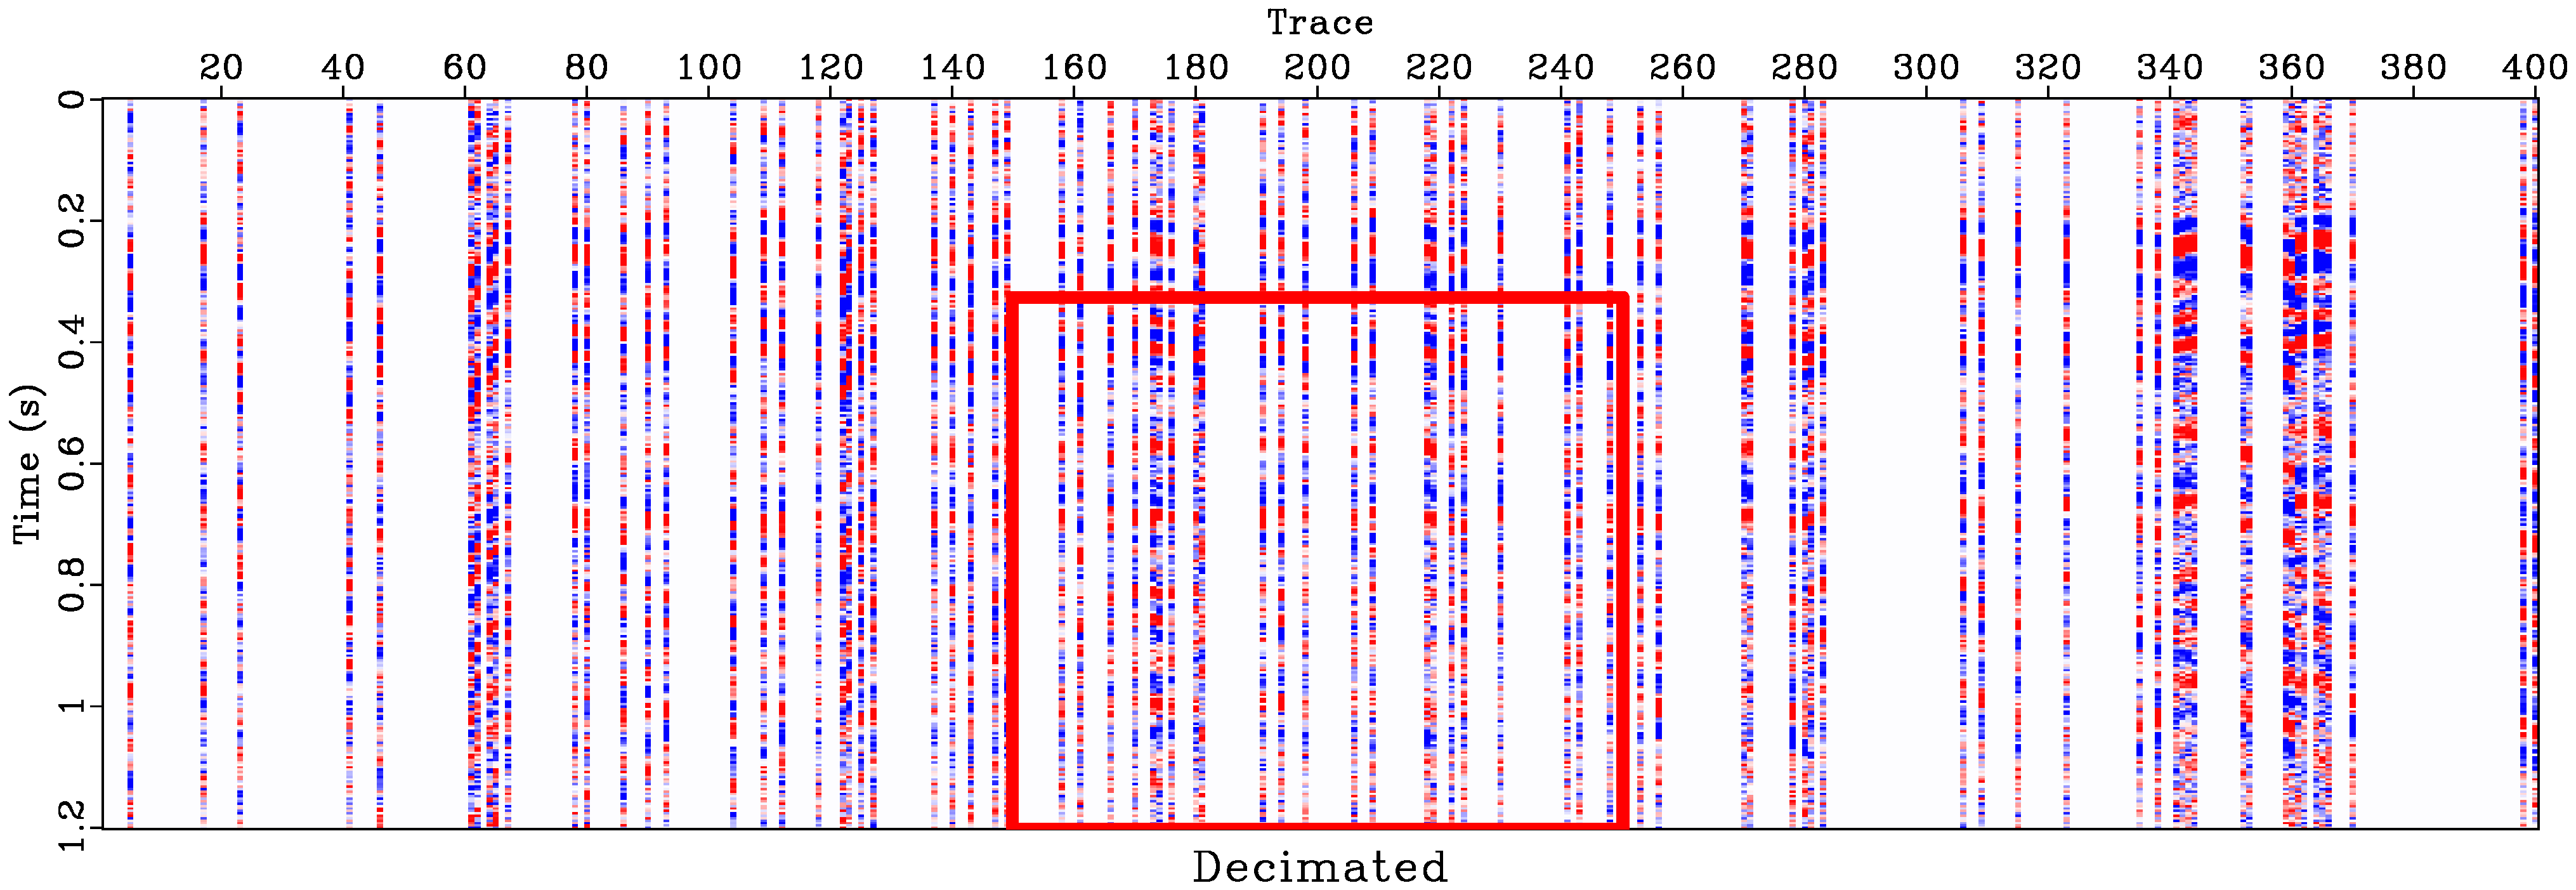
\includegraphics[width=\textwidth]{field/Fig/field5d-decimated2d-0}
    \label{fig:field5d-decimated2d-0}}
 \subfigure[]{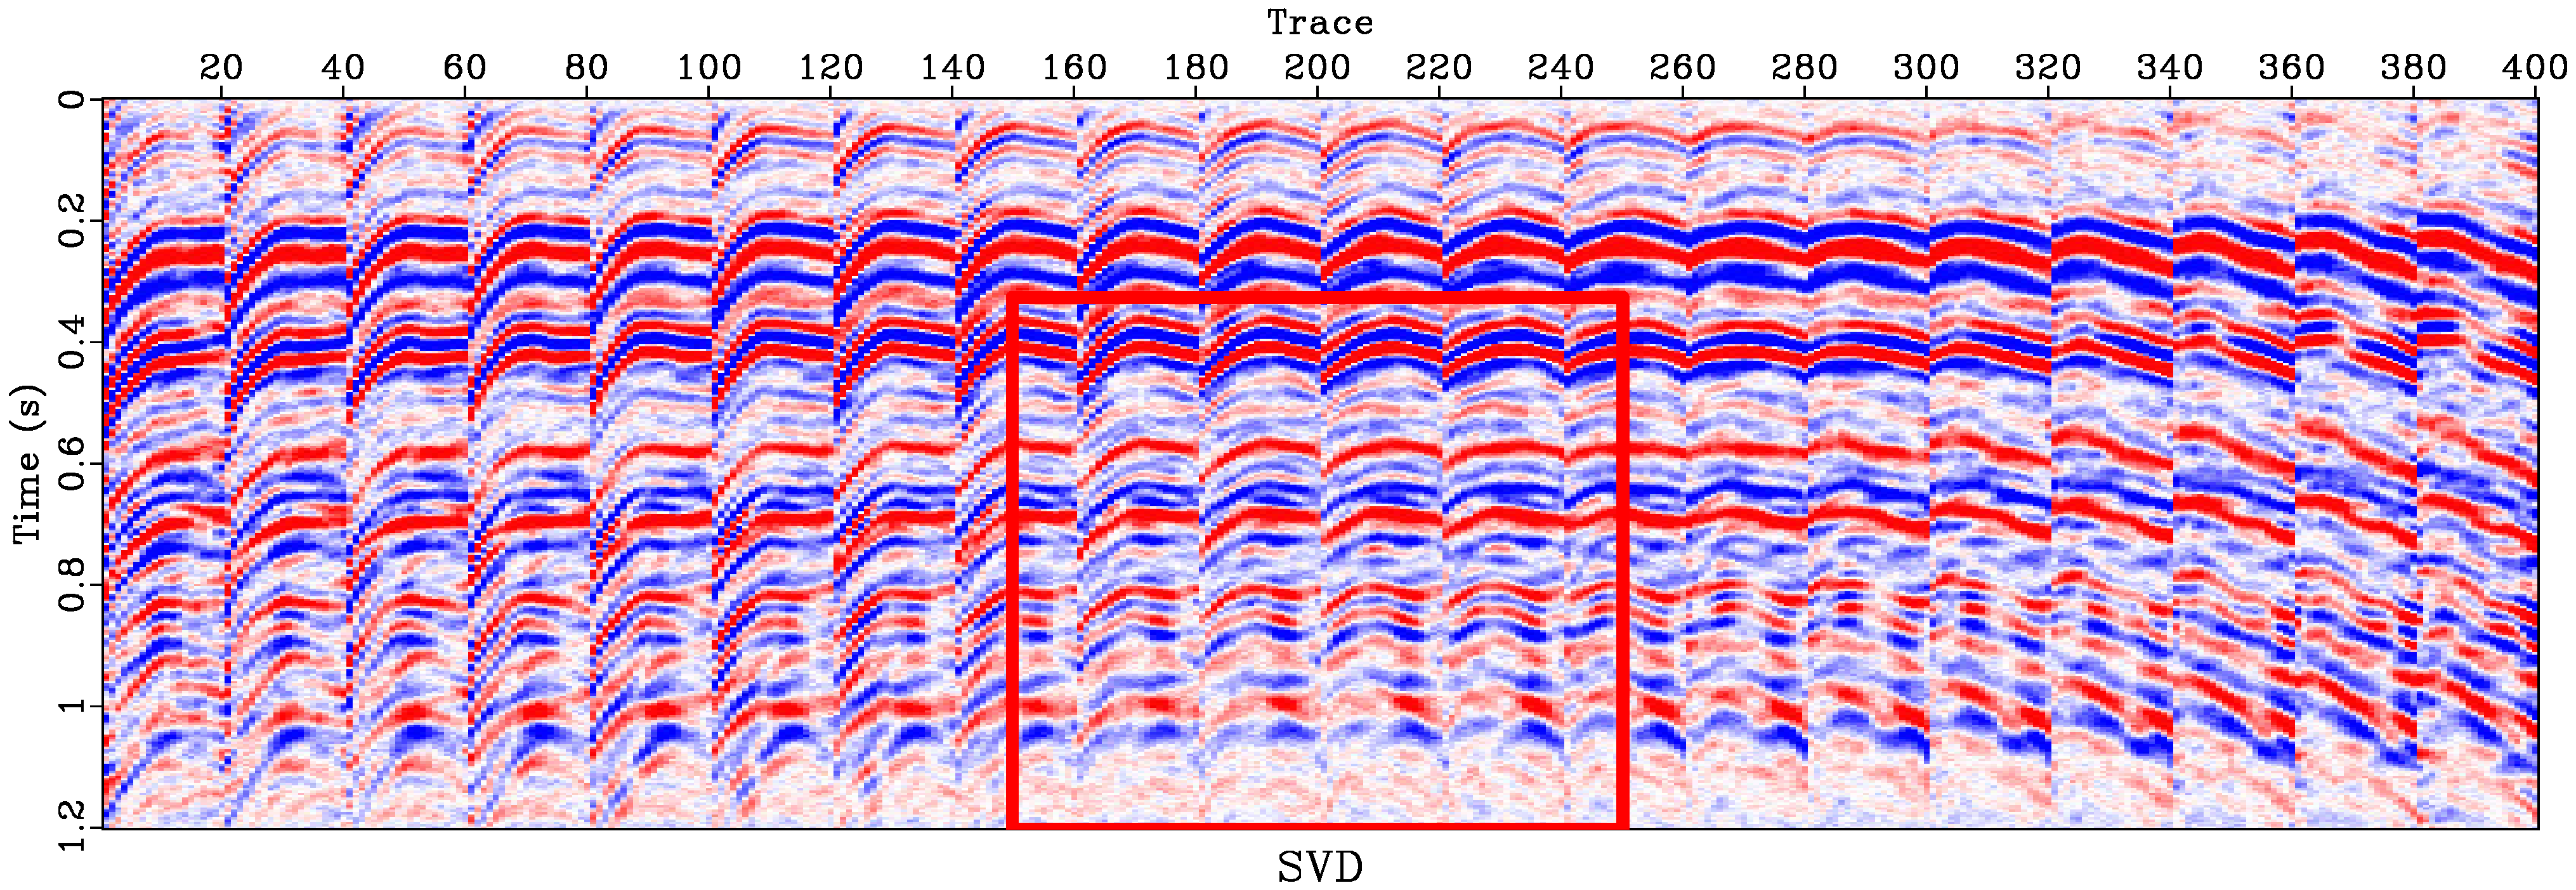
\includegraphics[width=\textwidth]{field/Fig/field5d-svd2d-0}
    \label{fig:field5d-svd2d-0}}
  \subfigure[]{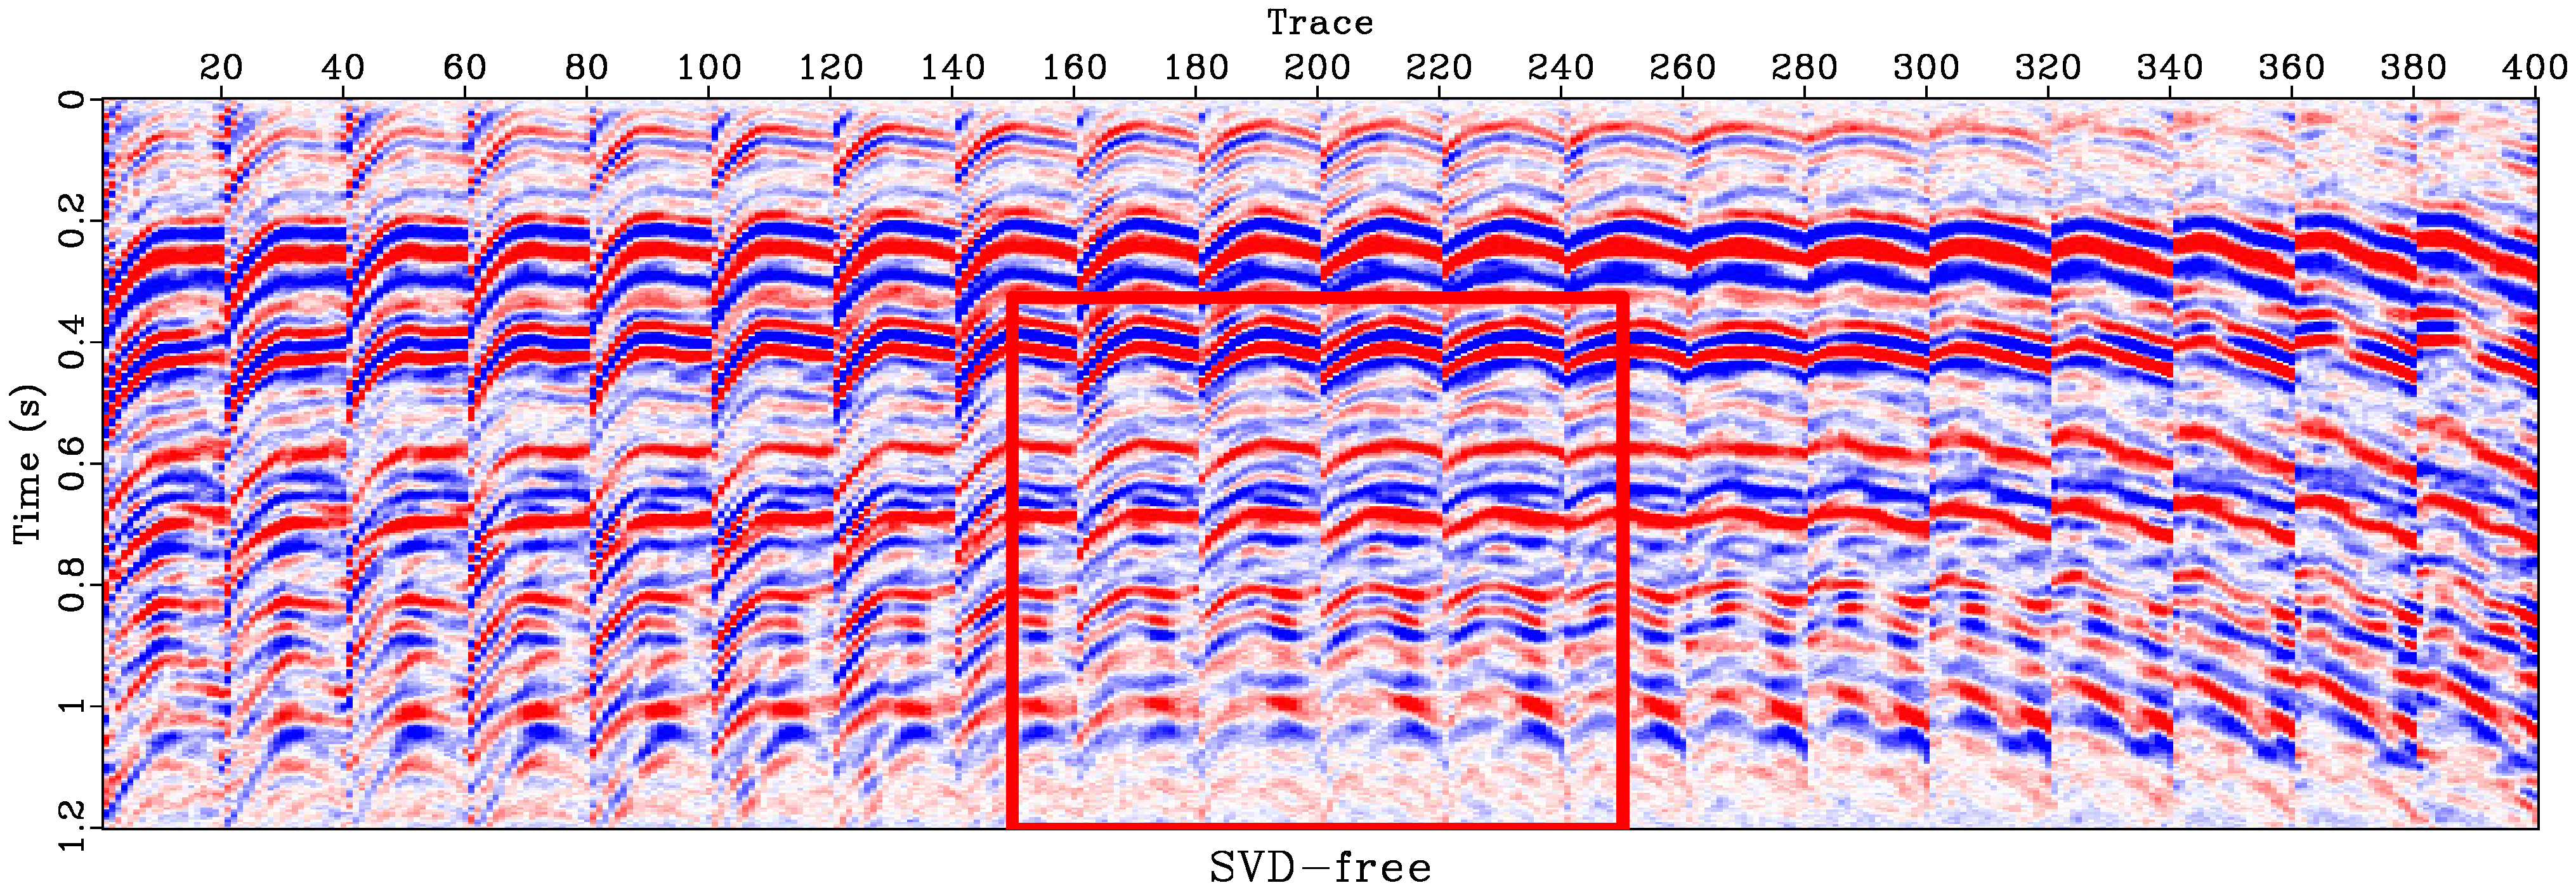
\includegraphics[width=\textwidth]{field/Fig/field5d-lmafit2d-0}
    \label{fig:field5d-lmafit2d-0}}
   \caption{Comparison of reconstruction performance in common offset gathers for the 5D field data example. (a) Observed data with roughly 80\% traces missing. (b) Reconstructed data using the SVD-based low-rank approximation method. (c) Reconstructed data using the SVD-free low-rank approximation method. The frame box areas are zoomed and highlighted in FIGURE \ref{fig:z-decimated,z-svd,z-lmafit}.}
\label{fig:field5d-decimated2d-0,field5d-svd2d-0,field5d-lmafit2d-0}
\end{figure*}

\begin{figure}[htb!]
  \centering
  \subfigure[]{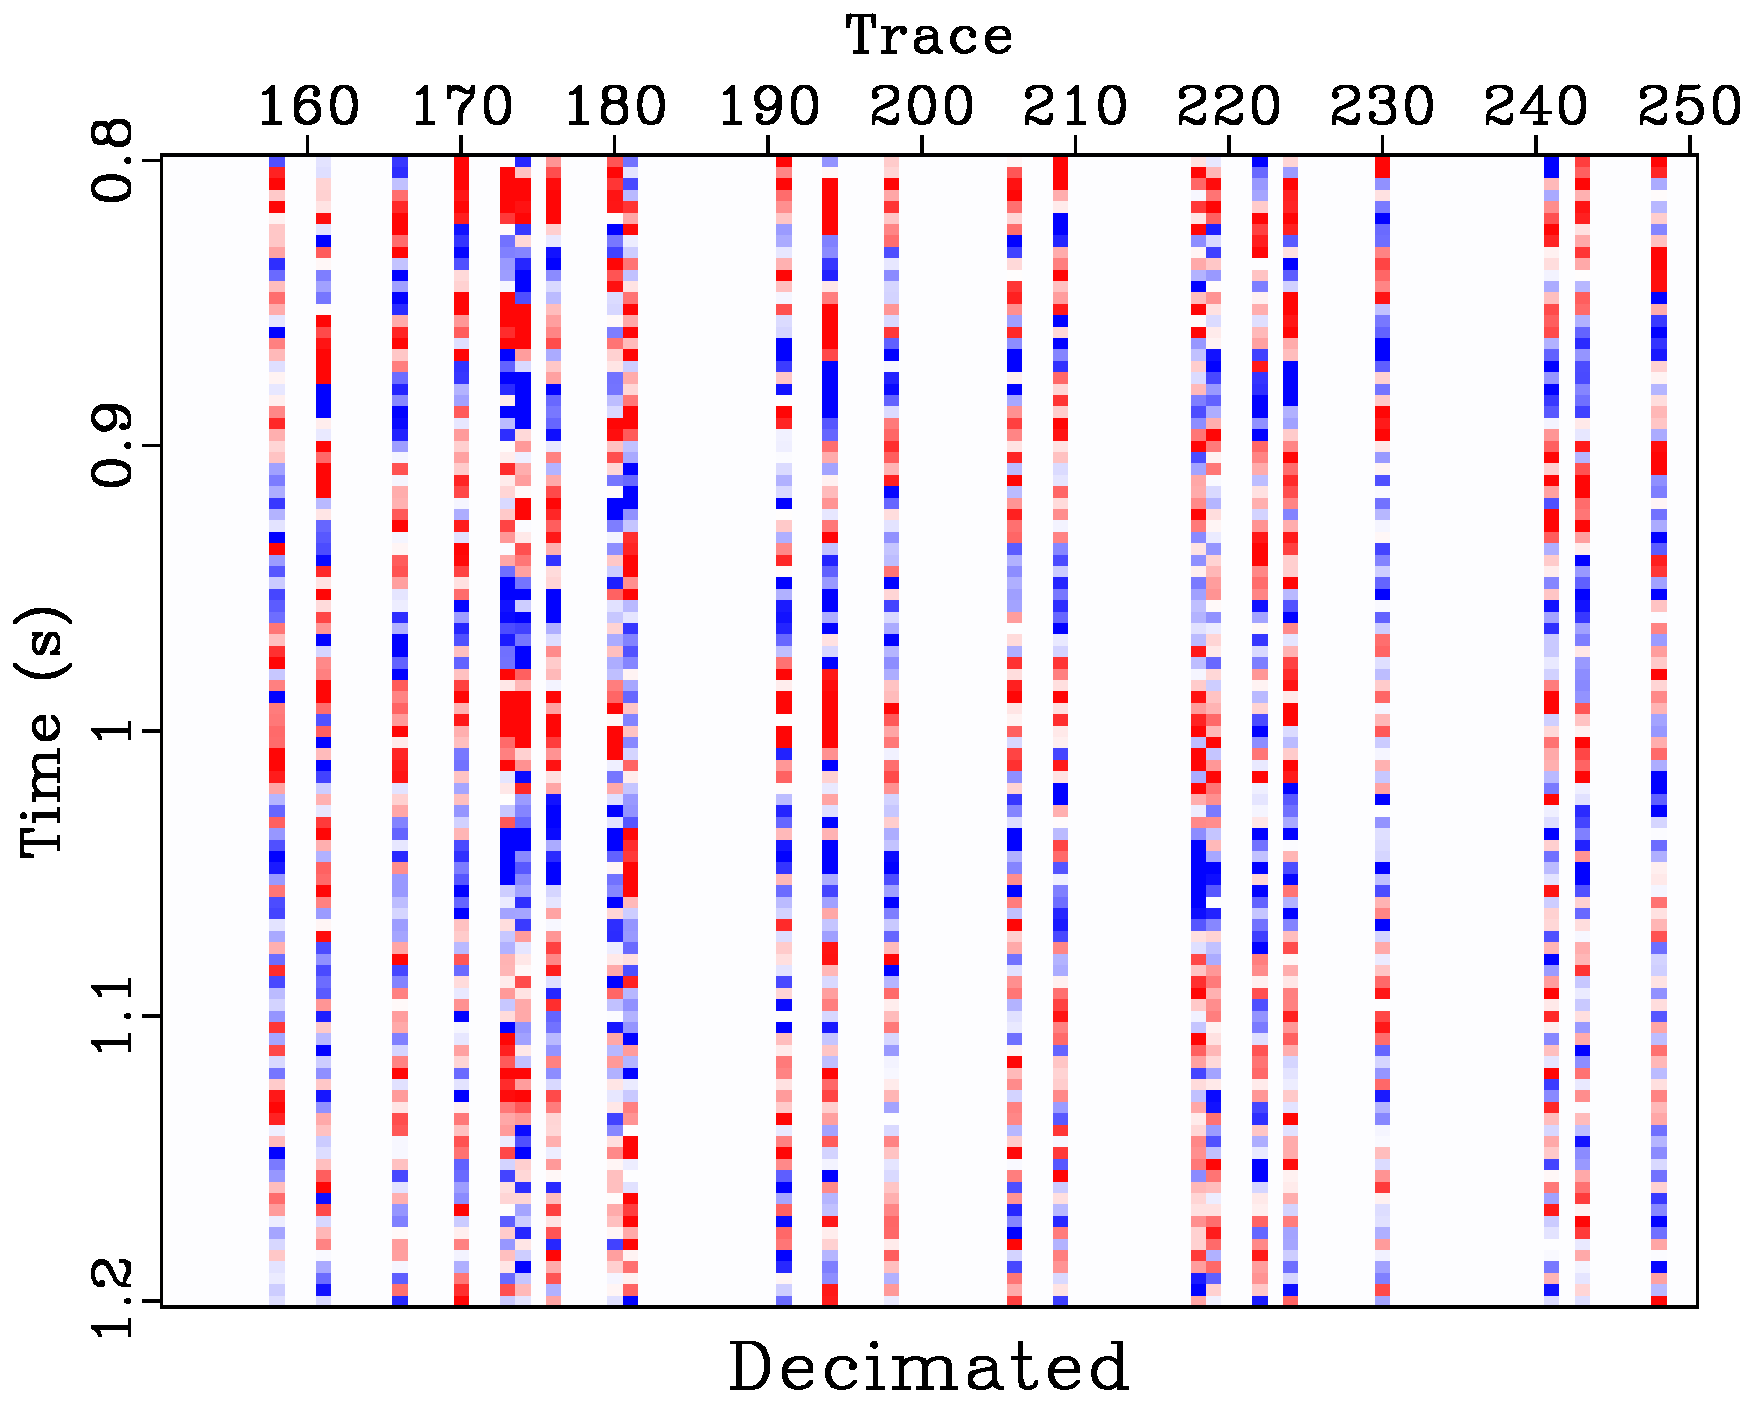
\includegraphics[width=0.9\columnwidth]{field/Fig/z-decimated}
    \label{fig:z-decimated}}
 \subfigure[]{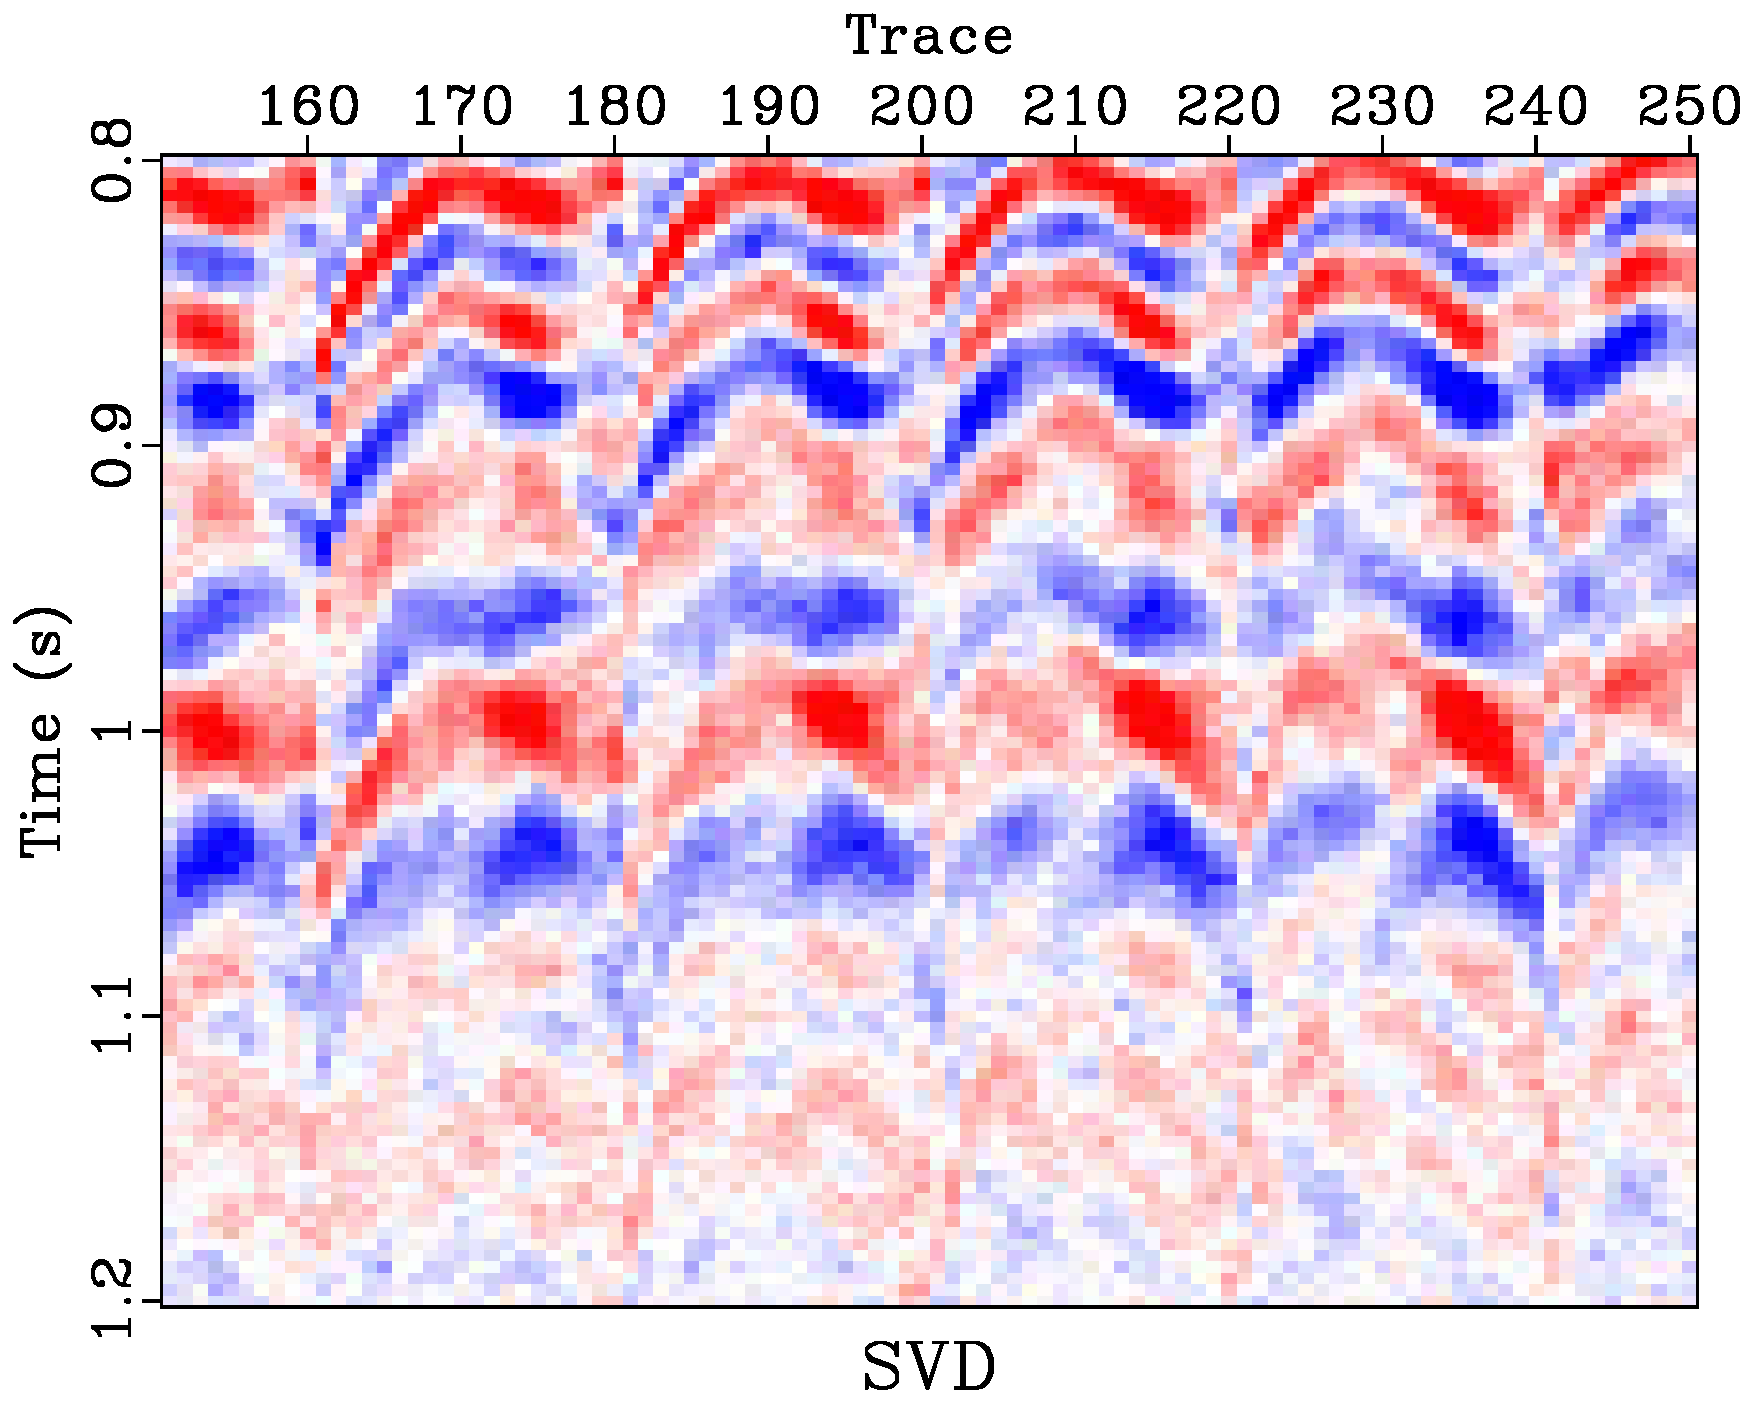
\includegraphics[width=0.9\columnwidth]{field/Fig/z-svd}
    \label{fig:z-svd}}
  \subfigure[]{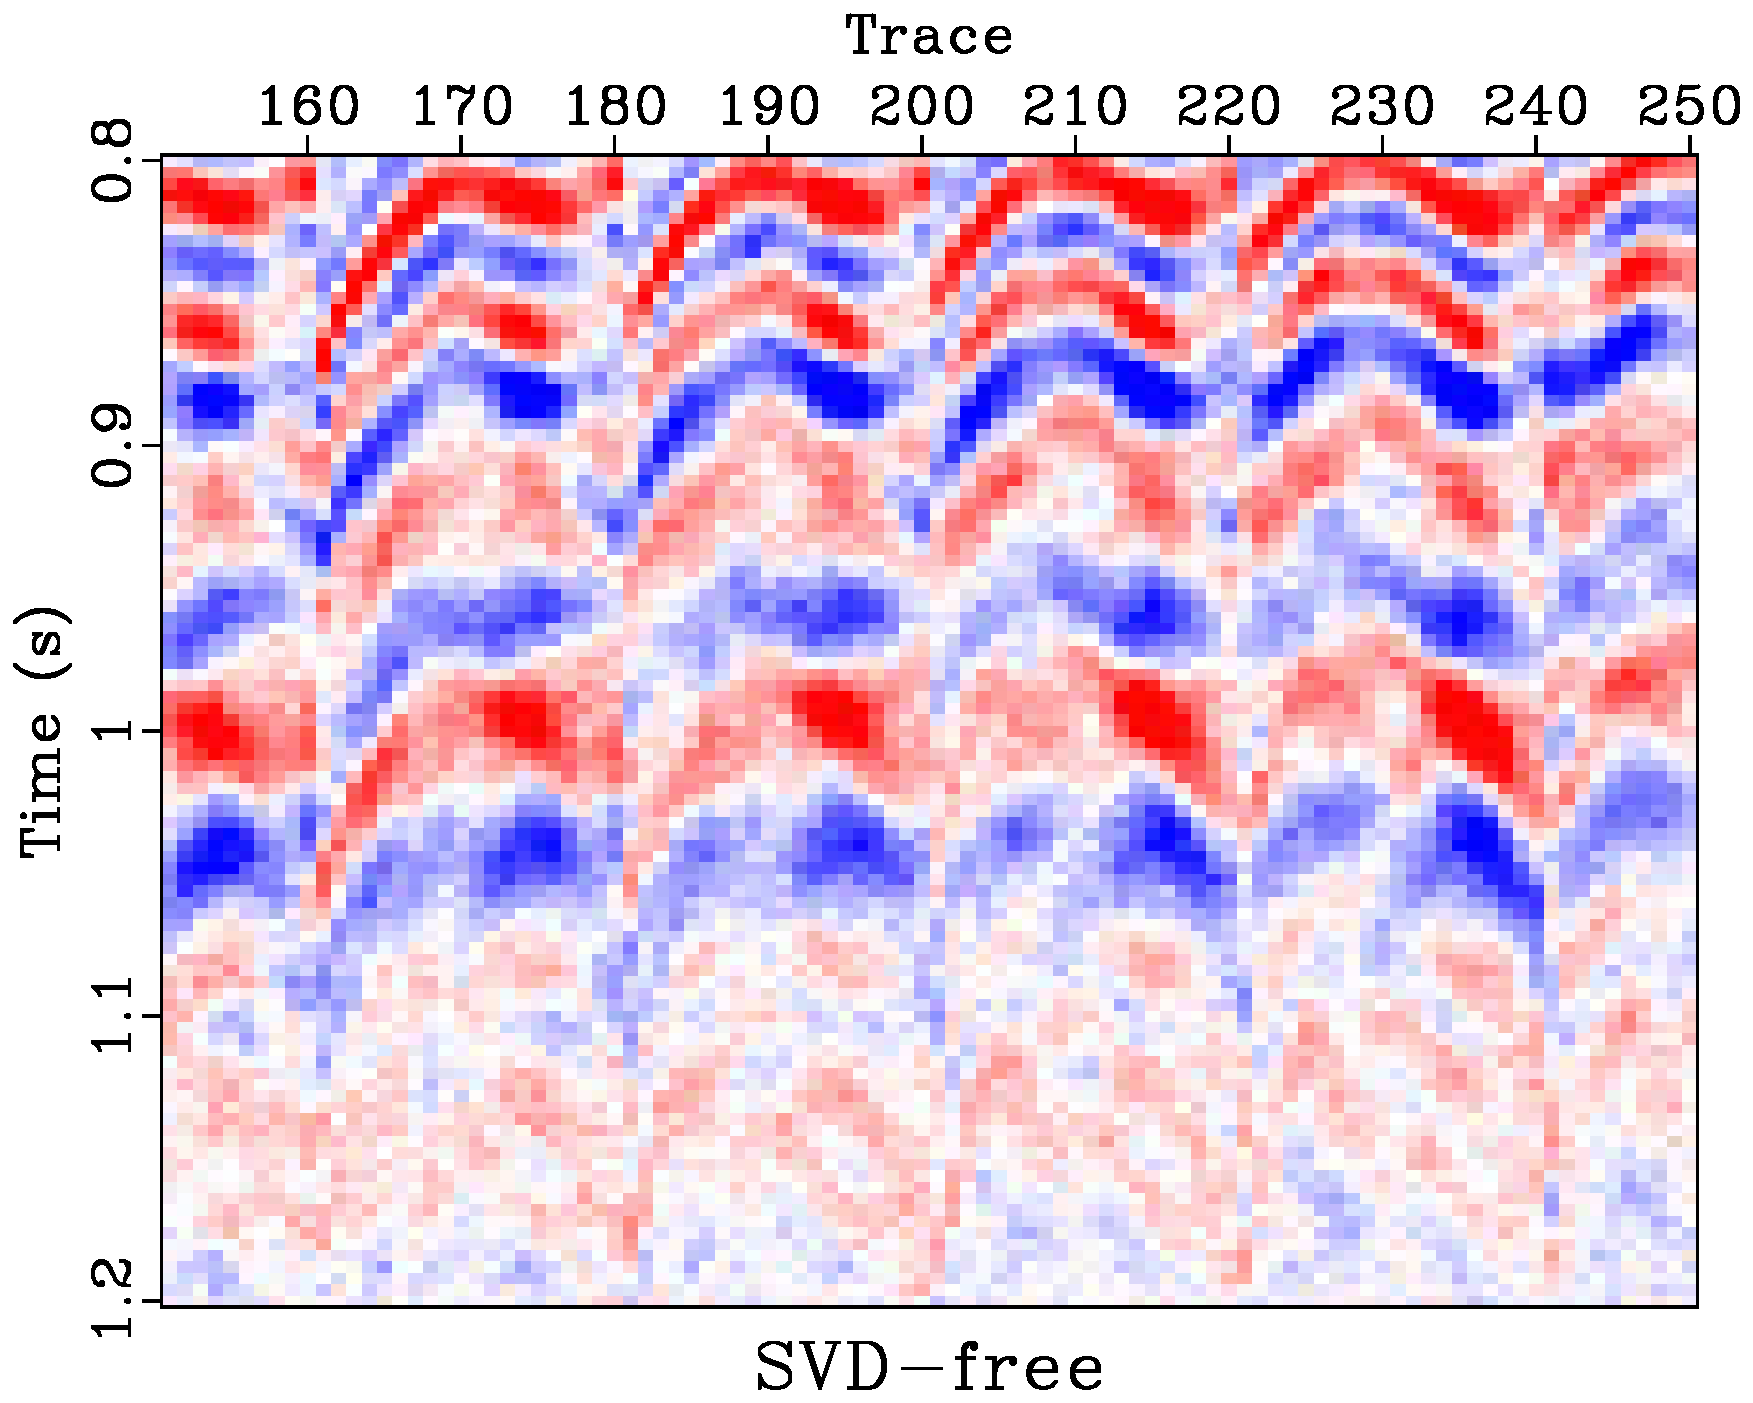
\includegraphics[width=0.9\columnwidth]{field/Fig/z-lmafit}
    \label{fig:z-lmafit}}
   \caption{Zoomed comparison of reconstruction performance in common offset gathers for the 5D field data example. (a) Observed data with roughly 80\% traces missing. (b) Reconstructed data using the SVD-based low-rank approximation method. (c) Reconstructed data using the SVD-free low-rank approximation method.}
\label{fig:z-decimated,z-svd,z-lmafit}
\end{figure}


%
%\inputdir{linear} % figure directory
%\multiplot{3}{syn5d-clean-3d,syn5d-noisy-3d,syn5d-decimated-3d}{width=0.28\textwidth}{Common offset gathers for the 5D synthetic example with linear events. (a) Clean data. (b) Noisy data. (c) The observed data with 80\% traces randomly removed. }
%
%\multiplot{6}{syn5d-svd-3d,syn5d-n-svd-3d,syn5d-r-svd-3d,syn5d-lmafit-3d,syn5d-n-lmafit-3d,syn5d-r-lmafit-3d}{width=0.28\textwidth}{Comparison of reconstruction performance in common offset gathers for the 5D synthetic example with linear events. (a) Reconstructed data using the SVD-based low-rank approximation method. (b) The removed noise from the noisy data corresponding to (a). (c) The reconstruction error corresponding to (a). (d) Reconstructed data using the SVD-free low-rank approximation method. (e) The removed noise from the noisy data corresponding to (d). (f) The reconstruction error corresponding to (d).}
%
%\multiplot{3}{syn5d-clean-3d-1,syn5d-noisy-3d-1,syn5d-decimated-3d-1}{width=0.28\textwidth}{Common midpoint gathers for the 5D synthetic example with linear events. (a) Clean data. (b) Noisy data. (c) The observed data with 80\% traces randomly removed.}
%
%\multiplot{6}{syn5d-svd-3d-1,syn5d-n-svd-3d-1,syn5d-r-svd-3d-1,syn5d-lmafit-3d-1,syn5d-n-lmafit-3d-1,syn5d-r-lmafit-3d-1}{width=0.28\textwidth}{Comparison of reconstruction performance in common midpoint gathers for the 5D synthetic example with linear events. (a) Reconstructed data using the SVD-based low-rank approximation method. (b) The removed noise from the noisy data corresponding to (a). (c) The reconstruction error corresponding to (a). (d) Reconstructed data using the SVD-free low-rank approximation method. (e) The removed noise from the noisy data corresponding to (d). (f) The reconstruction error corresponding to (d).}
%
%\multiplot{5}{syn5d-clean-2d,syn5d-noisy-2d,syn5d-decimated-2d,syn5d-svd-2d,syn5d-lmafit-2d}{width=0.28\textwidth}{Comparison of reconstruction performance in a 2D section. (a) Clean data. (b) Noisy data. (c) The observed data. (d) Reconstructed data using the SVD-based low-rank approximation method. (e) Reconstructed data using the SVD-free low-rank approximation method.}
%
%\inputdir{linear_time} 
%\plot{synth-ss}{width=0.9\columnwidth}{Comparison of the middle trace amplitude of each cubes in different datasets. The black line denotes the trace from the clean data.  The red line denotes the noisy data. The observed trace cannot be seen from this figure because it is a blank trace in the selection position. The SVD-based and SVD-free methods are denoted as blue and green lines, respectively. }%The yellow long-dashed line corresponds to $fl=10$ Hz. 
%%	The blue line corresponds to the traditional rank-reduction method. The green line corresponds to the proposed method. Note that the black and green lines are very close to each other, thus the reconstruction error using the proposed approach is much less than the traditional method for most parts.}
%
%\inputdir{linear} 
%\multiplot{4}{simi-syn5d-noisy-2d,simi-syn5d-decimated-2d,simi-syn5d-svd-2d,simi-syn5d-lmafit-2d}{width=0.34\textwidth}{Comparison of reconstruction performance in terms of local similarity. (a) Local similarity of the noisy data. (b) Local similarity of the observed data. (c) Local similarity of the reconstructed data using SVD-based low-rank approximation method. (d) Local similarity of the reconstructed data using SVD-free low-rank approximation method.}
%
%\inputdir{curve} % figure directory
%\multiplot{3}{curve5d-clean-3d-1,curve5d-noisy-3d-1,curve5d-decimated-3d-1}{width=0.28\textwidth}{Common midpoint gathers for the 5D synthetic example with hyperbolic events. (a) Clean data. (b) Noisy data. (c) The observed data with 80\% traces randomly removed. }
%
%\multiplot{6}{curve5d-svd-3d-1,curve5d-n-svd-3d-1,curve5d-r-svd-3d-1,curve5d-lmafit-3d-1,curve5d-n-lmafit-3d-1,curve5d-r-lmafit-3d-1}{width=0.28\textwidth}{Comparison of reconstruction performance in common midpoint gathers for the 5D synthetic example with hyperbolic events. (a) Reconstructed data using the SVD-based low-rank approximation method. (b) The removed noise from the noisy data corresponding to (a). (c) The reconstruction error corresponding to (a). (d) Reconstructed data using the SVD-free low-rank approximation method. (e) The removed noise from the noisy data corresponding to (d). (f) The reconstruction error corresponding to (d).}
%
%
%\multiplot{4}{simi-curve5d-noisy-3d-1,simi-curve5d-decimated-3d-1,simi-curve5d-svd-3d-1,simi-curve5d-lmafit-3d-1}{width=0.34\textwidth}{Comparison of reconstruction performance in terms of local similarity. (a) Local similarity of the noisy data. (b) Local similarity of the observed data. (c) Local similarity of the reconstructed data using SVD-based low-rank approximation method. (d) Local similarity of the reconstructed data using SVD-free low-rank approximation method.}


%\inputdir{./}
%\multiplot{2}{sr0,sr}{width=\textwidth}{\wen{(a) Source-receiver geometry for the SEG/EAGE salt synthetic data. (b) Source-receiver geometry for the decimated data. Red stars denote the shot positions. Blue inverted triangles denote the receiver positions.} }
%
%\multiplot{2}{sr00,sr11}{width=\textwidth}{\wen{(a) Source-receiver geometry for five representative shots without missing traces. (b) Source-receiver geometry for five representative shots with missing traces. Red stars denote the shot positions. Blue inverted triangles denote the receiver positions.} }

%\plot{bin}{width=0.8\textwidth}{\wen{Schematic plot demonstrating the data binning process (in a 2D surface view). The circles denote the binned regular grid points with (red) and without (green) waveform data. The black triangles denote the irregularly distributed receivers. Those within one grid distance to the nearby nodes contribute to the waveform stacking. The grid points without nearby stations are empty and need to be reconstructed.}}

%\inputdir{segeage}
%\multiplot{3}{seg0-3d-sxy,seg-svd-3d-sxy-rr,seg-svd-3d-sxy-lmafit}{width=0.45\textwidth}{\wen{Result of the SEG/EAGE salt example in common offset domain. (a) Incomplete data. (b) Reconstructed data using the SVD-based low-rank approximation method. (c) Reconstructed data using the SVD-free low-rank approximation method.} }
%
%\multiplot{3}{seg0-3d-hxy,seg-svd-3d-hxy-rr,seg-svd-3d-hxy-lmafit}{width=0.38\textwidth}{\wen{Result of the SEG/EAGE salt example in common shot-point domain. (a) Incomplete data. (b) Reconstructed data using the SVD-based low-rank approximation method. (c) Reconstructed data using the SVD-free low-rank approximation method.} }
%
%\multiplot{4}{seg0-2d-sxy-1,seg0-2d-sxy-2,seg1-2d-sxy-1,seg1-2d-sxy-2}{width=0.45\textwidth}{\wen{Comparison of 2D slices in common offset domain. (a) Incomplete data with SX=4340 m. (b) Reconstructed data with SX=4340 m using the proposed method. (c) Incomplete data with SX=5460 m. (d) Reconstructed data with SX=5460 m using the proposed method.} }
%
%\multiplot{4}{seg0-2d-sxy-3,seg0-2d-sxy-4,seg1-2d-sxy-3,seg1-2d-sxy-4}{width=0.38\textwidth}{\wen{Comparison of 2D slices in common offset domain. (a) Incomplete data with SY=3433 m. (b) Reconstructed data with SY=5845 m using the proposed method. (c) Incomplete data with SY=3433 m. (d) Reconstructed data with SX=5845 m using the proposed method.} }
%
%
%\multiplot{4}{seg0-2d-hxy-1,seg0-2d-hxy-2,seg1-2d-hxy-1,seg1-2d-hxy-2}{width=0.38\textwidth}{\wen{Comparison of 2D slices in common shot-point domain. (a) Incomplete data with HX=-100 m. (b) Reconstructed data with HX=20 m using the proposed method. (c) Incomplete data with HX=-100 m. (d) Reconstructed data with HX=20 m using the proposed method.} }
%
%\multiplot{4}{seg0-2d-hxy-3,seg0-2d-hxy-4,seg1-2d-hxy-3,seg1-2d-hxy-4}{width=0.45\textwidth}{\wen{Comparison of 2D slices in common shot-point domain. (a) Incomplete data with T=1.6 s (T denotes time). (b) Reconstructed data with T=2.4 s using the proposed method. (c) Incomplete data with T=1.6 s. (d) Reconstructed data with T=2.4 s using the proposed method.} }
%


%\renewcommand{\figdir}{field} % figure directory
%\inputdir{field}
%\multiplot{3}{field5d-decimated2d-0,field5d-svd2d-0,field5d-lmafit2d-0}{width=0.7\textwidth}{Comparison of reconstruction performance in common offset gathers for the 5D field data example. (a) Observed data with roughly 80\% traces missing. (b) Reconstructed data using the SVD-based low-rank approximation method. (c) Reconstructed data using the SVD-free low-rank approximation method. The frame box areas are zoomed and highlighted in Figure \ref{fig:z-decimated,z-svd,z-lmafit}.}
%
%\multiplot{3}{z-decimated,z-svd,z-lmafit}{width=0.45\textwidth}{Zoomed comparison of reconstruction performance in common offset gathers for the 5D field data example. (a) Observed data with roughly 80\% traces missing. (b) Reconstructed data using the SVD-based low-rank approximation method. (c) Reconstructed data using the SVD-free low-rank approximation method.}





\begin{table*}[h]
\caption{Comparison of computational cost of both the SVD-based and SVD-free low-rank approximation for different data sizes \wen{based on an Intel Core i7 CPU}.}
    \begin{center}
     \begin{tabular}{|c|c|c|c|} 
	  \hline Data size & $100\times10^4$  &  $100\times20^2\times10^2$  &   $300\times20^2\times10^2$ \\ 
	  \hline SVD-based (s) & 603 & 14320 & 92318 \\
      	  \hline SVD-free (s) & 153 & 2753 & 15302	       		 \\ 
          \hline
    \end{tabular} 
   \end{center}
\label{tbl:time}
\end{table*}


% 100*10*10*10*10: 	603,153
% 101*32*32*5*5: 	7226,1543
% 301*10*10*20*20: 	92340,15378
%

\new{\section{Synthetic examples}}
In this section, we use several\new{synthetic}  examples to demonstrate that the proposed SVD-free low-rank approximation method can significantly accelerate the reconstruction of 5D seismic data without loss of accuracy. \new{Although Hankel and Toeplitz matrices \cite{top1,top2} seem to be similar as the low-rank matrix, but in some cases one can lead us to better results in comparison to the other one. According to our experience, the Toeplitz matrix results in a slightly better reconstruction performance. So, here, we prefer to use the Toeplitz matrix as the low-rank matrix.} The first example is a synthetic example with linear events. We first construct a clean synthetic data, then we add some random noise to the data and also randomly remove some traces from the noisy data to simulate the incomplete seismic data. The size of this synthetic data is $100\times10\times10\times10\times10$. A comparison of the clean data, noisy data, and the incomplete data is presented in Figure \ref{fig:syn5d-clean-3d,syn5d-noisy-3d,syn5d-decimated-3d}, from which we can see that the added random noise is so strong that most useful seismic signals are not visible. Since 80\% of the total traces are removed from the original noisy data, the observed data is considered to be highly incomplete. We compare the reconstruction performance between the SVD-based low-rank approximation method and the SVD-free  low-rank approximation method in Figure \ref{fig:syn5d-svd-3d,syn5d-n-svd-3d,syn5d-r-svd-3d,syn5d-lmafit-3d,syn5d-n-lmafit-3d,syn5d-r-lmafit-3d}. The top row in Figure \ref{fig:syn5d-svd-3d,syn5d-n-svd-3d,syn5d-r-svd-3d,syn5d-lmafit-3d,syn5d-n-lmafit-3d,syn5d-r-lmafit-3d} corresponds to the results from the SVD-based low-rank approximation method and the bottom row in Figure \ref{fig:syn5d-svd-3d,syn5d-n-svd-3d,syn5d-r-svd-3d,syn5d-lmafit-3d,syn5d-n-lmafit-3d,syn5d-r-lmafit-3d} corresponds to the results from the SVD-free low-rank approximation method. In  Figure \ref{fig:syn5d-svd-3d,syn5d-n-svd-3d,syn5d-r-svd-3d,syn5d-lmafit-3d,syn5d-n-lmafit-3d,syn5d-r-lmafit-3d}, we show the reconstructed data in common offset gathers in the left column, the removed noise from the noisy data in the middle column, and the reconstruction error in the right column. The results show that the SVD-based and SVD-free low-rank approximation methods both obtain very successful reconstructions. The gaps in the observed incomplete data have been filled with seismic signals for both methods. The removed noise cubes of both methods do not contain obvious signal patterns, indicating that there are no significant damages to the useful signals during the reconstruction. The reconstruction error cubes also demonstrate that the error is negligible for both methods. However, for this example, the proposed SVD-free method is much faster than the SVD-based method. As tested on a Mac Pro Laptop equipped with an Intel Core i7 CPU clocked at 2.5 GHz and 16 GB of RAM, the SVD-based method takes 603 s to finish the calculation while the proposed only takes 153 s. The computational speedup is almost four times. A comparison of the computational efficiency of different methods for different data sizes is shown in Table \ref{tbl:time}.

The denoising performance in the common midpoint gathers is presented in Figures \ref{fig:syn5d-clean-3d-1,syn5d-noisy-3d-1,syn5d-decimated-3d-1} and \ref{fig:syn5d-svd-3d-1,syn5d-n-svd-3d-1,syn5d-r-svd-3d-1,syn5d-lmafit-3d-1,syn5d-n-lmafit-3d-1,syn5d-r-lmafit-3d-1}. Figure \ref{fig:syn5d-clean-3d-1,syn5d-noisy-3d-1,syn5d-decimated-3d-1} plots the clean synthetic data, noisy data, and decimated data with 80\% traces randomly removed. Figure \ref{fig:syn5d-svd-3d-1,syn5d-n-svd-3d-1,syn5d-r-svd-3d-1,syn5d-lmafit-3d-1,syn5d-n-lmafit-3d-1,syn5d-r-lmafit-3d-1} shows the reconstructed data, removed noise, and reconstruction error cubes using the SVD-based and SVD-free low-rank approximation methods. A single-slice comparison in the common offset gather is presented in Figure \ref{fig:syn5d-clean-2d,syn5d-noisy-2d,syn5d-decimated-2d,syn5d-svd-2d,syn5d-lmafit-2d}. From the single-slice comparison, we can see that both methods obtain very similar results (Figures \ref{fig:syn5d-svd-2d} and \ref{fig:syn5d-lmafit-2d}), which are very close to the clean data (Figure \ref{fig:syn5d-clean-2d}). To numerically compare the reconstruction performance, we use the signal-to-noise ratio (SNR) defined as follows \cite{weilin2016,weilin2017gji}:
\begin{equation}
\label{eq:dsnr}
SNR=10\log_{10}\frac{\Arrowvert \mathbf{s} \Arrowvert_2^2}{\Arrowvert \mathbf{s} -\hat{\mathbf{s}}\Arrowvert_2^2}.
\end{equation}
where $\mathbf{s}$ denotes the vectorized clean data and $\hat{\mathbf{s}}$ denotes the vectorized reconstructed data. 

To further compare the amplitude difference among different datasets, we extract a single trace from each data cubes of the clean, noisy, observed, and reconstructed data using two methods. The trace to be compared is the middle trace in each dataset. The single-trace comparison is plotted in Figure \ref{fig:synth-ss}. The clean data is plotted as the black line. The noisy data is plotted as the red line. The observed data is not plotted because in this position it is a blank trace. The blue line plots the trace using the SVD-based low-rank approximation method. The green line plots the trace using the SVD-free method. It is apparent that both SVD-based and SVD-free methods obtain very successful recovery of the exact solution, i.e., the clean trace. Although there are tiny differences between the blue and the green lines, they are overall very similar. 


The calculated SNR of the incomplete data is -8.08 dB. The SNRs of the SVD-based and SVD-free low-rank approximation methods are \old{9.49 dB and 9.64 dB}\new{9.53 dB and 9.79 dB}, respectively. We find that the proposed SVD-free low-rank approximation can even obtain a slight improvement in terms of SNR. Besides, we also use the local similarity metric \cite{yangkang2015ortho} to compare the reconstruction performance of different methods. Figure \ref{fig:simi-syn5d-noisy-2d,simi-syn5d-decimated-2d,simi-syn5d-svd-2d,simi-syn5d-lmafit-2d} shows the comparison of local similarity maps of different datasets. Figure \ref{fig:simi-syn5d-noisy-2d} plots the local similarity between clean data and the noisy data, where we can see that the high local similarity is consistent with the distribution of the useful signals. Although, it is difficult to observe signals from the very noisy data, it is possible to use local similarity to highlight the distribution of the useful signals in the presence of extremely strong random noise. Figure \ref{fig:simi-syn5d-decimated-2d} shows the local similarity map between the observed incomplete data and the clean data. The right side of the section has distinctly zero local similarity value, due to the missing traces. Figures \ref{fig:simi-syn5d-svd-2d} and \ref{fig:simi-syn5d-lmafit-2d} show the local similarity maps corresponding to the SVD-based and SVD-free low-rank approximation methods. The very close local similarity maps of two methods indicate that the reconstruction performance is nearly the same. 



Next, we use a synthetic example with hyperbolic events to test the performance of the proposed method in the case of curved events. The clean data, noisy data, and incomplete data with 80\% missing traces are shown in Figure \ref{fig:curve5d-clean-3d-1,curve5d-noisy-3d-1,curve5d-decimated-3d-1}. The size of this synthetic data is $101\times32\times32\times5\times5$.  The comparison of reconstruction results using the SVD-based and SVD-free methods is presented in Figure \ref{fig:curve5d-svd-3d-1,curve5d-n-svd-3d-1,curve5d-r-svd-3d-1,curve5d-lmafit-3d-1,curve5d-n-lmafit-3d-1,curve5d-r-lmafit-3d-1}. The left column in Figure \ref{fig:curve5d-svd-3d-1,curve5d-n-svd-3d-1,curve5d-r-svd-3d-1,curve5d-lmafit-3d-1,curve5d-n-lmafit-3d-1,curve5d-r-lmafit-3d-1} plots the reconstructed data. The middle column in Figure \ref{fig:curve5d-svd-3d-1,curve5d-n-svd-3d-1,curve5d-r-svd-3d-1,curve5d-lmafit-3d-1,curve5d-n-lmafit-3d-1,curve5d-r-lmafit-3d-1} plots the removed noise. The right column in Figure \ref{fig:curve5d-svd-3d-1,curve5d-n-svd-3d-1,curve5d-r-svd-3d-1,curve5d-lmafit-3d-1,curve5d-n-lmafit-3d-1,curve5d-r-lmafit-3d-1} plots the reconstruction error. From Figure \ref{fig:curve5d-svd-3d-1,curve5d-n-svd-3d-1,curve5d-r-svd-3d-1,curve5d-lmafit-3d-1,curve5d-n-lmafit-3d-1,curve5d-r-lmafit-3d-1}, it is clear that both methods obtain very similar performance. However, the computational costs for the SVD-based and SVD-free methods are 7226 s, and 1543s, respectively. Figure \ref{fig:simi-curve5d-noisy-3d-1,simi-curve5d-decimated-3d-1,simi-curve5d-svd-3d-1,simi-curve5d-lmafit-3d-1}
shows the comparison of local similarity cubes. Figure \ref{fig:simi-curve5d-noisy-3d-1} plots the local similarity between the noisy data and the clean data. Figure \ref{fig:simi-curve5d-decimated-3d-1} plots the local similarity between the observed incomplete data and the clean data. Figure \ref{fig:simi-curve5d-svd-3d-1} plots the local similarity between the reconstructed data and the clean data using the SVD-based low-rank approximation method. Figure \ref{fig:simi-curve5d-lmafit-3d-1} plots the local similarity between the reconstructed data and the clean data using the SVD-free low-rank approximation method. From the similarity cubes, we see that the reconstructions from both methods help recover most of the useful signals and obtain high local similarity measures. The performance of the SVD-free method is further confirmed to be close to the SVD-based method in terms of local similarity measure. The SNRs of the reconstructed data using the SVD-based method and the SVD-free method are \old{1.72 dB and 1.89 dB}\new{1.75 dB and 1.92 dB}, respectively. Note that the SNR of the incomplete data of this example is extremely low, i.e., -13.73 dB. This example also demonstrates the effectiveness of the SVD-free low-rank approximation method in the case of ultra-low SNR. 

\new{\section{Real data example}}
Finally, we apply the proposed SVD-free low-rank approximation method to a 5D field data. The data have been binned onto a regular grid and a common offset gather of the field data is shown in Figure \ref{fig:field5d-decimated2d-0,field5d-svd2d-0,field5d-lmafit2d-0}. In Figure \ref{fig:field5d-decimated2d-0,field5d-svd2d-0,field5d-lmafit2d-0}, the \old{coloured}\new{colored} stripes are the recorded seismic traces. The white blanks denote the missing traces, which means that we do not observe seismic data in these positions. The size of this field data is $301\times10\times10\times20\times20$. Because of the difficulty in displaying a 5D data set, we only show a common mid-point gather here. The 3D common midpoint gather is re-arranged into a 2D matrix for a better view. The transparent \old{coloured}\new{colored} windows denote zooming areas for an amplified comparison. In this example, roughly 80 percent traces are missing from the regular grids. Because of the high ratio of missing traces, the observed seismic traces do not show any spatial coherency. It is difficult to see the waveforms from the raw data. The results from the two aforementioned methods, i.e., SVD-based and SVD-free methods, are shown in Figures \ref{fig:field5d-svd2d-0} and \ref{fig:field5d-lmafit2d-0}. After 5D reconstruction, the white blanks in the raw data have been filled with seismic traces. The waveforms become well aligned along the spatial direction. Compared with the raw data, all methods seem to obtain a dramatic improvement on the data quality. It is salient that both low-rank approximation methods obtain much smoother and cleaner results.  When zooming the data in the transparent red rectangles in both Figures \ref{fig:field5d-svd2d-0} and \ref{fig:field5d-lmafit2d-0}, the comparison among different datasets becomes much clearer. From Figure \ref{fig:z-decimated,z-svd,z-lmafit}, we observe that both low-rank approximation methods obtain very similar results. In this example, the SVD-free method takes 15378 s while the SVD-based method takes 92340 s. The speedup using the proposed SVD-free low-rank approximation is nearly six times. 


\section{Conclusion}
The traditional singular value decomposition (SVD) based low-rank approximation method suffers from the bottleneck of computational cost due to many SVD calculations. In order to relieve the computation overburden, we develop an SVD-free low-rank approximation method in this paper. The SVD-free matrix decomposition is based on an alternating minimization strategy. During the iterative update, we only need a much faster QR factorization for solving a linear least-squares problem. The SVD-free low-rank approximation can be easily inserted into the singular spectrum analysis (SSA) framework. We test the effectiveness of the SVD-free method on synthetic examples with linear and curving events,  and a real 5D seismic data. The results show that the proposed SVD-free method do not degrade the reconstruction performance compared with the traditional method. However, the proposed SVD-free method can greatly improve the computational efficiency. 


\begin{thebibliography}{00}
\bibitem{ronen}
J.~Ronen, ``Wave-equation trace interpolation,'' \emph{Geophysics}, vol.~52,
  pp. 973--984, 1987.

\bibitem{spitz1991}
S.~Spitz, ``Seismic trace interpolation in the f-x domain,'' \emph{Geophysics},
  vol.~56, pp. 785--794, 1991.

\bibitem{chen1995}
J.~Chen and J.~Cihlar, ``Quantifying the effect of canopy architecture on
  optical measurements of leaf area index using two gap size analysis
  methods,'' \emph{IEEE Transactions on Geoscience and Remote Sensing},
  vol.~33, pp. 777--787, 1995.

\bibitem{canning1996}
A.~Canning and G.~H.~F. Gardner, ``Reducing 3{D} acquisition footprint for 3{D}
  dmo and 3{D} prestack migration,'' \emph{Geophysics}, vol.~63, pp.
  1177--1183, 1996.

\bibitem{fomel2002pwd}
S.~Fomel, ``Application of plane-wave destruction filters,'' \emph{Geophysics},
  vol.~67, pp. 1946--1960, 2002.

\bibitem{fomel2003}
------, ``Seismic reflection data interpolation with differential offset and
  shot continuation,'' \emph{Geophysics}, vol.~68, pp. 733--744, 2003.

\bibitem{abmapocs}
R.~Abma and N.~Kabir, ``\protect{3D} interpolation of irregular data with a
  \protect{POCS} algorithm,'' \emph{Geophysics}, vol.~71, pp. E91--E97, 2006.

\bibitem{herrmann2008non}
F.~J. Herrmann and G.~Hennenfent, ``Non-parametric seismic data recovery with
  curvelet frames,'' \emph{Geophysical Journal International}, vol. 173, no.~1,
  pp. 233--248, 2008.

\bibitem{protter2009}
M.~Protter and M.~Elad, ``Image sequence denoising via sparse and redundant
  representations,'' \emph{IEEE Trans Image Process}, vol.~18, no.~1, pp.
  27--35, 2009.

\bibitem{mostafa2010}
M.~Naghizadeh and M.~D. Sacchi, ``Beyond alias hierarchical scale curvelet
  interpolation of regularly and irregularly sampled seismic data,''
  \emph{Geophysics}, vol.~75, p. WB189–WB202, 2010.

\bibitem{mostafa2013}
------, ``Multidimensional de-aliased cadzow reconstruction of seismic
  records,'' \emph{Geophysics}, vol.~78, no.~1, pp. A1--A5, 2010.

\bibitem{wang2011recovery}
Y.~Wang, J.~Cao, and C.~Yang, ``Recovery of seismic wavefields based on
  compressive sensing by an l 1-norm constrained trust region method and the
  piecewise random subsampling,'' \emph{Geophysical Journal International},
  vol. 187, no.~1, pp. 199--213, 2011.

\bibitem{yanan2014}
Y.~Tian, Y.~Li, and B.~Yang, ``Variable-eccentricity hyperbolic-trace {TFPF}
  for seismic random noise attenuation,'' \emph{IEEE Transactions on Geoscience
  and Remote Sensing}, vol.~52, pp. 6449--6458, 2014.

\bibitem{yanhui2016}
Y.~Zhou, J.~Gao, W.~Chen, and P.~Frossard, ``Seismic simultaneous source
  separation via patchwise sparse representation,'' \emph{IEEE Transactions on
  Geoscience and Remote Sensing}, vol.~54, pp. 5271--5284, 2016.

\bibitem{kazemi2016}
N.~Kazemi, E.~Bongajum, and M.~D. Sacchi, ``Surface-consistent sparse
  multichannel blind deconvolution of seismic signals,'' \emph{IEEE
  Transactions on Geoscience and Remote Sensing}, vol.~54, pp. 3200--3207,
  2016.
\bibitem{shuwei2016cs}
S.~Gan, S.~Wang, Y.~Chen, X.~Chen, W.~Huang, and H.~Chen, ``Compressive sensing
  for seismic data reconstruction via fast projection onto convex sets based on
  seislet transform,'' \emph{Journal of Applied Geophysics}, vol. 130, pp.
  194--208, 2016.

\bibitem{lorenzi2016}
L.~Lorenzi, F.~Melgani, and G.~Mercier, ``Missing-area reconstruction in
  multispectral images under a compressive sensing perspective,'' \emph{IEEE
  Transactions on Geoscience and Remote Sensing}, vol.~51, pp. 3998--4008,
  2016.

\bibitem{shaohuan2016gap}
S.~Zu, H.~Zhou, Y.~Chen, X.~Pan, S.~Gan, and D.~Zhang, ``Interpolating big gaps
  using inversion with slope constraint,'' \emph{IEEE Geoscience and Remote
  Sensing Letters}, vol.~13, pp. 1369--1373, 2016.

\bibitem{yangkang2016irr5d}
Y.~Chen, D.~Zhang, Z.~Jin, X.~Chen, S.~Zu, W.~Huang, and S.~Gan, ``Simultaneous
  denoising and reconstruction of 5{D} seismic data via damped rank-reduction
  method,'' \emph{Geophysical Journal International}, vol. 206, pp. 1695--1717,
  2016.

\bibitem{amir2017ieee}
R.~Anvari, M.~A.~N. Siahsar, S.~Gholtashi, A.~R. Kahoo, and M.~Mohammadi,
  ``Seismic random noise attenuation using synchrosqueezed wavelet transform
  and low-rank signal matrix approximation,'' \emph{IEEE Transactions on
  Geoscience and Remote Sensing}, vol.~55, no.~11, pp. 6574--6581, 2017.

\bibitem{verschuure1991}
D.~J. Verschuur, ``Surface-related multiple elimination: An inversion
  approach,'' \emph{PhD thesis, Delft University of Technology}, 1991.

\bibitem{jingjie2011review}
J.~Cao, Y.~Wang, J.~Zhao, and C.~Yang, ``A review on restoration of seismic
  wavefields based on regularization and compressive sensing,'' \emph{Inverse
  Problems in Science and Engineering}, vol.~19, no.~5, pp. 679--704, 2011.

\bibitem{yangkang20142}
Y.~Chen, S.~Fomel, and J.~Hu, ``Iterative deblending of simultaneous-source
  seismic data using seislet-domain shaping regularization,''
  \emph{Geophysics}, vol.~79, pp. V179--V189, 2014.

\bibitem{shuwei20153}
S.~Gan, S.~Wang, Y.~Chen, Y.~Zhang, and Z.~Jin, ``Dealiased seismic data
  interpolation using seislet transform with low-frequency constraint,''
  \emph{IEEE Geoscience and Remote Sensing Letters}, vol.~12, pp. 2150--2154,
  2015.

\bibitem{shuwei2016vscan}
S.~Gan, S.~Wang, Y.~Chen, S.~Qu, and S.~Zu, ``Velocity analysis of
  simultaneous-source data using high-resolution semblance-coping with the
  strong noise,'' \emph{Geophysical Journal International}, vol. 204, pp.
  768--779, 2016.

\bibitem{liuwei2016dealiase}
W.~Liu, S.~Cao, S.~Gan, Y.~Chen, S.~Zu, and Z.~Jin, ``One-step slope estimation
  for dealiased seismic data reconstruction via iterative seislet
  thresholding,'' \emph{IEEE Geoscience and Remote Sensing Letters}, vol.~13,
  pp. 1462--1466, 2016.

\bibitem{shaohuan2017gji}
S.~Zu, H.~Zhou, W.~Mao, D.~Zhang, C.~Li, X.~Pan, and Y.~Chen, ``Iterative
  deblending of simultaneous-source data using a coherency-pass shaping
  operator,'' \emph{Geophysical Journal International}, vol. 211, no.~1, pp.
  541--557, 2017.

\bibitem{YuSiwei2015}
S.~Yu, J.~Ma, X.~Zhang, and M.~D. Sacchi, ``Interpolation and denoising of
  high-dimensional seismic data by learning a tight frame,'' \emph{Geophysics},
  vol.~80, no.~5, pp. V119--V132, 2015. [Online]. Available:
  \url{https://doi.org/10.1190/geo2014-0396.1}


\bibitem{YuSiwei2016}
S.~Yu, J.~Ma, and S.~Osher, ``Monte carlo data-driven tight frame for seismic
  data recovery,'' \emph{Geophysics}, vol.~81, no.~4, pp. V327--V340, 2016.
  [Online]. Available: \url{https://doi.org/10.1190/geo2015-0343.1}


\bibitem{Jia2017}
Y.~Jia and J.~Ma, ``What can machine learning do for seismic data processing?
  an interpolation application,'' \emph{Geophysics}, vol.~82, no.~3, pp.
  V163--V177, 2017. [Online]. Available:
  \url{https://doi.org/10.1190/geo2016-0300.1}


\bibitem{amir2017sp}
M.~A.~N. Siahsar, V.~Abolghasemi, and Y.~Chen, ``Simultaneous denoising and
  interpolation of 2{D} seismic data using data-driven non-negative dictionary
  learning,'' \emph{Signal Processing}, vol. 141, pp. 309--321, 2017.

\bibitem{amir2017geo}
M.~A.~N. Siahsar, S.~Gholtashi, A.~R. Kahoo, W.~Chen, and Y.~Chen,
  ``Data-driven multi-task sparse dictionary learning for noise attenuation of
  3{D} seismic data,'' \emph{Geophysics}, vol.~82, no.~6, p. V385–V396, 2017.

\bibitem{Jia2018}
Y.~Jia, S.~Yu, and J.~Ma, ``Intelligent interpolation by monte carlo machine
  learning,'' \emph{Geophysics}, vol.~83, no.~2, pp. V83--V97, 2018. [Online].
  Available: \url{https://doi.org/10.1190/geo2017-0294.1}


\bibitem{zhangmi2019}
M.~Zhang, Y.~Liu, M.~Bai, and Y.~Chen, ``Seismic noise attenuation using
  unsupervised sparse feature learning,'' \emph{IEEE Transactions on Geoscience
  and Remote Sensing}, p. doi: 10.1109/TGRS.2019.2928715, 2019.

\bibitem{yangkang2015ortho}
Y.~Chen and S.~Fomel, ``Random noise attenuation using local signal-and-noise
  orthogonalization,'' \emph{Geophysics}, vol.~80, pp. WD1--WD9, 2015.

\bibitem{guochang2012}
G.~Liu, X.~Chen, J.~Du, and K.~Wu, ``Random noise attenuation using \emph{f-x}
  regularized nonstationary autoregression,'' \emph{Geophysics}, vol.~77, pp.
  V61--V69, 2012.

\bibitem{fxnaghizadeh}
M.~Naghizadeh and M.~Sacchi, ``Multicomponent f-x seismic random noise
  attenuation via vector autoregressive operators,'' \emph{Geophysics},
  vol.~77, pp. V91--V99, 2012.

\bibitem{beckouche}
S.~Beckouche and J.~Ma, ``Simultaneous dictionary learning and denoising for
  seismic data,'' \emph{Geophysics}, vol.~79, pp. A27--A31, 2014.

\bibitem{mostafa2016bssa}
S.~M. Mousavi and C.~A. Langston, ``Hybrid seismic denoising using higher-order
  statistics and improved wavelet block thresholding,'' \emph{Bulletin of the
  Seismological Society of America}, vol. 106, no.~4, pp. 1380--1393, 2016.

\bibitem{mostafa2017geo}
------, ``Automatic noise-removal/signal-removal based on general
  cross-validation thresholding in synchrosqueezed domain and its application
  on earthquake data,'' \emph{Geophysics}, vol.~82, no.~4, pp. V211--V227,
  2017.

\bibitem{zhaoqiang2018}
Q.~Zhao, Q.~Du, X.~Gong, and Y.~Chen, ``Signal-preserving erratic noise
  attenuation via iterative robust sparsity-promoting filter,'' \emph{IEEE
  Transactions on Geoscience and Remote Sensing}, vol.~56, no.~6, pp.
  1558--0644, 2018.

\bibitem{oropezamssa}
V.~Oropeza and M.~Sacchi, ``Simultaneous seismic data denoising and
  reconstruction via multichannel singular spectrum analysis,''
  \emph{Geophysics}, vol.~76, pp. V25--V32, 2011.

\bibitem{gaomssa}
J.~Gao, M.~Sacchi, and X.~Chen, ``A fast reduced-rank interpolation method for
  prestack seismic volumes that depend on four spatial dimensions,''
  \emph{Geophysics}, vol.~78, pp. V21--V30, 2013.

\bibitem{Gaogp}
J.~Gao, A.~Stanton, M.~Naghizadeh, M.~D. Sacchi, and X.~Chen, ``Convergence
  improvement and noise attenuation considerations for beyond alias projection
  onto convex sets reconstruction,'' \emph{Geophysical Prospecting}, vol.~61,
  pp. 138--151, 2013.

\bibitem{gholami}
A.~Gholami, ``Non-convex compressed sensing with frequency mask for seismic
  data reconstruction and denoising,'' \emph{Geophysical Prospecting}, vol.~62,
  pp. 1389--1405, 2015.

\bibitem{benfengpocs}
B.~Wang, R.~Wu, X.~Chen, and J.~Li, ``Simultaneous seismic data interpolation
  and denoising with a new adaptive method based on dreamlet transform,''
  \emph{Geophysical Journal International}, vol. 201, pp. 1180--1192, 2015.

\bibitem{pmf}
J.~Gao, A.~Stanton, and M.~D. Sacchi, ``Parallel matrix factorization algorithm
  and its application to 5{D} seismic reconstruction and denoising,''
  \emph{Geophysics}, vol.~80, pp. V173--V187, 2015.

\bibitem{wangchong2018}
C.~Wang, Z.~Zhu, H.~Gu, X.~Wu, and S.~Liu, ``Hankel low-rank approximation for
  seismic noise attenuation,'' \emph{IEEE Transactions on Geoscience and Remote
  Sensing}, no.~99, pp. 1--13, 2018.

\bibitem{Liubin2004}
B.~Liu and M.~D. Sacchi, ``Minimum weighted norm interpolation of seismic
  records,'' \emph{Geophysics}, vol.~69, no.~6, pp. 1560--1568, 2004. [Online].
  Available: \url{https://doi.org/10.1190/1.1836829}


\bibitem{Trad2007}
D.~Trad, ``A strategy for wide azimuth land interpolation,'' \emph{SEG
  Technical Program Expanded Abstracts}, pp. 946--950, 2007. [Online].
  Available: \url{https://library.seg.org/doi/abs/10.1190/1.2792562}


\bibitem{Trad2009}
------, ``Five-dimensional interpolation: Recovering from acquisition
  constraints,'' \emph{Geophysics}, vol.~74, pp. V123--V132, 2009.

\bibitem{GaoJianjun2017}
J.~Gao, J.~Cheng, and M.~D. Sacchi, ``Five-dimensional seismic reconstruction
  using parallel square matrix factorization,'' \emph{IEEE Transactions on
  Geoscience and Remote Sensing}, vol.~55, no.~4, pp. 2124--2135, April 2017.

\bibitem{Xie2017}
Y.~Xie and D.~Gajewski, ``5-{D} interpolation with wavefront attributes,''
  \emph{Geophysical Journal International}, vol. 211, pp. 897--919, 08 2017.

\bibitem{lu2015fast}
L.~Lu, W.~Xu, and S.~Qiao, ``A fast {SVD} for multilevel block hankel matrices
  with minimal memory storage,'' \emph{Numerical Algorithms}, vol.~69, no.~4,
  pp. 875--891, 2015.

\bibitem{jinkun2016}
J.~Cheng and M.~Sacchi, ``Fast dual-domain reduced-rank algorithm for 3{D}
  deblending via randomized qr decomposition,'' \emph{Geophysics}, vol.~81, pp.
  V89--V101, 2014.

\bibitem{jianjun2017five}
J.~Gao, J.~Cheng, and M.~D. Sacchi, ``Five-dimensional seismic reconstruction
  using parallel square matrix factorization,'' \emph{IEEE Transactions on
  Geoscience and Remote Sensing}, vol.~55, no.~4, pp. 2124--2135, 2017.

\bibitem{gavish2014optimal}
M.~Gavish and D.~L. Donoho, ``The optimal hard threshold for singular values is
  4/sqrt(3),'' \emph{IEEE Transactions on Information Theory}, vol.~60, no.~8,
  pp. 5040--5053, 2014.

\bibitem{trickett2015preserving}
S.~Trickett, ``Preserving signal: Automatic rank determination for noise
  suppression,'' in \emph{SEG Technical Program Expanded Abstracts 2015}.\hskip
  1em plus 0.5em minus 0.4em\relax Society of Exploration Geophysicists, 2015,
  pp. 4703--4707.

\bibitem{aharchaou2017singular}
M.~Aharchaou, J.~Anderson, S.~Hughes, and J.~Bingham, ``Singular-spectrum
  analysis via optimal shrinkage of singular values,'' in \emph{SEG Technical
  Program Expanded Abstracts 2017}.\hskip 1em plus 0.5em minus 0.4em\relax
  Society of Exploration Geophysicists, 2017, pp. 4950--4954.

\bibitem{yatong2018gji}
Y.~Zhou, S.~Li, D.~Zhang, and Y.~Chen, ``Seismic noise attenuation using an
  online subspace tracking algorithm,'' \emph{Geophysical Journal
  International}, vol. 212, no.~2, p. 1072–1097, 2018.

\bibitem{wujuan2018jge3}
J.~Wu and M.~Bai, ``Adaptive rank-reduction method for seismic data
  reconstruction,'' \emph{Journal of Geophysics and Engineering}, vol.~15, p.
  1688, 2018.

\bibitem{weilin2016}
W.~Huang, R.~Wang, Y.~Chen, H.~Li, and S.~Gan, ``Damped multichannel singular
  spectrum analysis for 3{D} random noise attenuation,'' \emph{Geophysics},
  vol.~81, no.~4, pp. V261--V270, 2016.

\bibitem{weilingieeedls}
W.~Huang, R.~Wang, X.~Chen, and Y.~Chen, ``Double least-squares projections
  method for signal estimation,'' \emph{IEEE Transactions on Geoscience and
  Remote Sensing}, vol.~55, pp. 4111--4129, 2017.

\bibitem{dong}
D.~Zhang, Y.~Chen, W.~Huang, and S.~Gan, ``Multi-step damped multichannel
  singular spectrum analysis for simultaneous reconstruction and denoising of
  3{D} seismic data,'' \emph{Journal of Geophysics and Engineering}, vol.~13,
  pp. 704--720, 2016.

\bibitem{dong2017}
D.~Zhang, Y.~Zhou, H.~Chen, W.~Chen, S.~Zu, and Y.~Chen, ``Hybrid rank-sparsity
  constraint model for simultaneous reconstruction and denoising of 3{D}
  seismic data,'' \emph{Geophysics}, vol.~82, pp. V351--V367, 2017.

\bibitem{yufeng2017}
Y.~Wang, H.~Zhou, S.~Zu, W.~Mao, and Y.~Chen, ``Three-operator proximal
  splitting scheme for 3{D} seismic data reconstruction,'' \emph{IEEE
  Geoscience and Remote Sensing Letters}, vol.~14, no.~10, pp. 1830--1834,
  2017.

\bibitem{yangkangelra}
Y.~Chen, Y.~Zhou, W.~Chen, S.~Zu, W.~Huang, and D.~Zhang, ``Empirical low-rank
  approximation for seismic noise attenuation,'' \emph{IEEE Transactions on
  Geoscience and Remote Sensing}, vol.~55, pp. 4696--4711, 2017.

\bibitem{baimin2018cg}
M.~Bai, J.~Wu, S.~Zu, and W.~Chen, ``A structural rank reduction operator for
  removing artifacts in least-squares reverse time migration,'' \emph{Computers
  and Geosciences}, vol. 117, pp. 9--20, 2018.

\bibitem{stanton2013processing}
A.~Stanton, N.~Kazemi, and M.~D. Sacchi, ``Processing seismic data in the
  presence of residual statics,'' in \emph{SEG Technical Program Expanded
  Abstracts 2013}.\hskip 1em plus 0.5em minus 0.4em\relax Society of
  Exploration Geophysicists, 2013, pp. 1838--1842.

\bibitem{lmafit}
Z.~Wen, W.~Yin, and Y.~Zhang, ``Solving a low-rank factorization model for
  matrix completion by a nonlinear successive over-relaxation algorithm,''
  \emph{Mathematical Programming Computation}, vol.~4, pp. 333--361, 2012.

\bibitem{weilin2017gji}
W.~Huang, R.~Wang, S.~Zu, and Y.~Chen, ``Low-frequency noise attenuation in
  seismic and microseismic data using mathematical morphological filtering,''
  \emph{Geophysical Journal International}, vol. 211, p. 1318–1340, 2017.

\bibitem{yangkang2020odrr}
Y.~Chen, M.~Bai, Z.~Guan, Q. Zhang, M. Zhang, and H.~Wang, ``Five-dimensional seismic data reconstruction using the optimally damped rank-reduction method,''
  \emph{Geophysical Journal International}, vol. 222, p. 1824-1845, 2020.
  
\bibitem{top1}
A.~Bottcher, S.M.~Grudsky, and T.~Kunz, ``Toeplitz Matrices, Asymptotic Linear Algebra, and Functional Analysis,''
  \emph{ISBN: 978-3-7643-6290-4,A Birkhäuser book}, 2000.
  
\bibitem{top2}
R.M.~Gray, ``Toeplitz and Circulant Matrices: A review,''
  \emph{Foundations and Trends in Communications and Information Theory}, vol. 2, pp. 155-239, 2006.



\end{thebibliography}

%\begin{IEEEbiography}[{\includegraphics[width=1in,height=1.25in,clip,keepaspectratio]{a1.png}}]{First A. Author} (M'76--SM'81--F'87) and all authors may include 
%biographies. Biographies are often not included in conference-related
%papers. This author became a Member (M) of IEEE in 1976, a Senior
%Member (SM) in 1981, and a Fellow (F) in 1987. The first paragraph may
%contain a place and/or date of birth (list place, then date). Next,
%the author's educational background is listed. The degrees should be
%listed with type of degree in what field, which institution, city,
%state, and country, and year the degree was earned. The author's major
%field of study should be lower-cased. 
%
%The second paragraph uses the pronoun of the person (he or she) and not the 
%author's last name. It lists military and work experience, including summer 
%and fellowship jobs. Job titles are capitalized. The current job must have a 
%location; previous positions may be listed 
%without one. Information concerning previous publications may be included. 
%Try not to list more than three books or published articles. The format for 
%listing publishers of a book within the biography is: title of book 
%(publisher name, year) similar to a reference. Current and previous research 
%interests end the paragraph. The third paragraph begins with the author's 
%title and last name (e.g., Dr.\ Smith, Prof.\ Jones, Mr.\ Kajor, Ms.\ Hunter). 
%List any memberships in professional societies other than the IEEE. Finally, 
%list any awards and work for IEEE committees and publications. If a 
%photograph is provided, it should be of good quality, and 
%professional-looking. Following are two examples of an author's biography.
%\end{IEEEbiography}
%
%\begin{IEEEbiography}[{\includegraphics[width=1in,height=1.25in,clip,keepaspectratio]{a2.png}}]{Second B. Author} was born in Greenwich Village, New York, NY, USA in 
%1977. He received the B.S. and M.S. degrees in aerospace engineering from 
%the University of Virginia, Charlottesville, in 2001 and the Ph.D. degree in 
%mechanical engineering from Drexel University, Philadelphia, PA, in 2008.
%
%From 2001 to 2004, he was a Research Assistant with the Princeton Plasma 
%Physics Laboratory. Since 2009, he has been an Assistant Professor with the 
%Mechanical Engineering Department, Texas A{\&}M University, College Station. 
%He is the author of three books, more than 150 articles, and more than 70 
%inventions. His research interests include high-pressure and high-density 
%nonthermal plasma discharge processes and applications, microscale plasma 
%discharges, discharges in liquids, spectroscopic diagnostics, plasma 
%propulsion, and innovation plasma applications. He is an Associate Editor of 
%the journal \emph{Earth, Moon, Planets}, and holds two patents. 
%
%Dr. Author was a recipient of the International Association of Geomagnetism 
%and Aeronomy Young Scientist Award for Excellence in 2008, and the IEEE 
%Electromagnetic Compatibility Society Best Symposium Paper Award in 2011. 
%\end{IEEEbiography}
%
\clearpage
\begin{IEEEbiography}[{\includegraphics[width=1in,height=1.25in,clip,keepaspectratio]{juan}}]{Juan Wu} received the Ph.D. degree in geophysics from the China University of Petroleum, Beijing, China, in 2016, under the supervision of Prof. Xiaohong Chen.
She is currently a Post-Doctoral Researcher with Yangtze University, Jingzhou, China. She has authored or coauthored more than 30 journal articles. Her research interests include seismic signal analysis and seismic imaging.
\end{IEEEbiography}

\begin{IEEEbiography}[{\includegraphics[width=1in,height=1.25in,clip,keepaspectratio]{min}}]{Min Bai}
 received the Ph.D. degree in geophysics from the China University of Petroleum, Beijing, China, in 2016, under the supervision of Prof. Xiaohong Chen.
He is currently a Post-Doctoral Researcher with the School of Earth Sciences, Zhejiang University, Hangzhou, China, and a Lecturer with Yangtze University, Jingzhou, China. He has authored or coauthored more than 30 journal articles. His research interests include seismic imaging and inversion and seismic signal analysis.
\end{IEEEbiography}




\begin{IEEEbiography}[{\includegraphics[width=1in,height=1.25in,clip,keepaspectratio]{dong}}]{Dong Zhang} received the B.S. degree in applied geophysics from Jilin University, Changchun, China, in 2014.  He is currently pursuing a PhD degree in Geophysics at Delft university of technology. His current research interests include seismic signal analysis, seismic imaging and simultaneous-source data deblending and imaging.
\end{IEEEbiography}

\begin{IEEEbiography}[{\includegraphics[width=1in,height=1.25in,clip,keepaspectratio]{hang}}]{Hang Wang} received a master degree in geological resources and geological engineering from China University of Petroleum (Beijing), and he is a Ph.D. candidate in geophysics at Zhejiang University. His research interests include seismic signal processing, machine learning and FWI.
\end{IEEEbiography}


\begin{IEEEbiography}[{\includegraphics[width=1in,height=1.25in,clip,keepaspectratio]{guangtan}}]{Guangtan Huang} received the B.S., M.S., and Ph.D. degrees in exploration geophysics from the China University of Petroleum (East China), Beijing, Beijing, China, in 2012, 2015, and 2019, respec- tively. He holds a post-doctoral position in geophyiscs at Zhejiang University, Hangzhou, China. His research interests include seismic forward modeling and high-resolution seismic inversion.
\end{IEEEbiography}



\begin{IEEEbiography}[{\includegraphics[width=1in,height=1.25in,clip,keepaspectratio]{yangkang}}]{Yangkang Chen} received the B.S. degree in explo- ration geophysics from the China University of Petroleum, Beijing, Beijing, China, in 2012, and the Ph.D. degree in geophysics from the University of Texas at Austin, Austin, TX, USA, in 2015, under the supervision of Prof. S. Fomel.
He was a Distinguished Post-Doctoral Research Associate with Oak Ridge National Laboratory, Oak Ridge, TN, USA, where he conducted research on global adjoint tomography. He is an Assistant Pro- fessor with Zhejiang University, Hangzhou, China. He has authored or coauthored more than 100 internationally renowned journal articles and more than 80 international conference papers. His research interests include seismic signal analysis, seismic modeling and inversion, simultaneous-source data deblending and imaging, global adjoint tomography, machine learning, and high-performance computing.
\end{IEEEbiography}

\EOD


